\section{Background Estimation}
\label{sec:analysis:background}





This analysis has three main sources of backgrounds:

\begin{itemize}
    \item vector boson plus jets
    \item multijet QCD
    \item diboson production
\end{itemize}

Vector boson (W or Z) production is the most prominent source of backgrounds overall.  These processes are well modelled and the simulation is found to be sufficient for the precision of modelling we require.  Diboson production is similarily well modelled, but is far less significant.  

It is worth pointing out that normalization of the W+jet, WW, and WZ production will all be sensitive to variations of the \PW decay branching fractions.  In general the yield from these processes are very small compared to \ttbar and tW production.  It is also the case that we assume fairly conservative uncertainties on the normalization of these processes ($\geq 5\%$) such that there should not be any sensitivity to the effect of the variation of the branching fractions.  For the case of the shape analysis, the \PW + jets sample is treated as a signal sample and is decomposed based on the decay modes of the \PW boson.  

The multijet QCD background affects the $e\tau$, $e$ + jets, $\mu\tau$, and $\mu$ + jets channels.  The number of generated events for this process is found to be insufficient for accurately modelling the event yields and shapes for this process so data-driven methods are employed.

The breakdown of predicted backgrounds are shown in tables~\ref{tab:yields} and \ref{tab:yields_ltau}.   


In several of the selected channels there is a non-negligible contamination from non-prompt production of leptons, in particular, the channels targetting semi-leptonic \ttbar decays and decays with hadronic taus in the final state.  One production process that gives rise to these events for which there is insufficient MC events is multiplepton QCD.  These events tend to affect selections where there is only one electron or muon.  This background is estimated using two different methods: for the semileptonic \ttbar selections, an estimate based on the fake rate method is used; for the hadronic $\tau$ final states, a sideband selected by inverting the dilepton charge requirement is used for the estimate.




\subsection{Fake rate method}

A commonly used method for estimating backgrounds from misidentified prompt lepton production can be summarized as follows:

\begin{enumerate}
    \item construct a control region that is enhanced in the production of leptons from non-prompt sources,
    
    \item measure the ratio, the ``fake rate", of the number of leptons passing a loose selection criteria to the number passing a tighter selection, i.e., the number of muons passing the analysis isolation requirement to those that pass with no isolation requirement,
    
        \begin{equation}
            f = \frac{N_{\rm pass\ iso}}{N_{\rm no iso}}
        \end{equation}

    \item apply a weight based on the fake rate ($w = f/(1-f)$) to events in the signal region where the leptons are required to pass the loose requirement but fail the tight requirement.
\end{enumerate}

The control region that is used for the fake rate measurement is selected to be enhanced in \PZ plus jet production.  Specifically, it is required that:

\begin{itemize}
    \item there are at least two muons or electrons passing the full analysis requirements,
    \item the two leptons must have opposite signs,
    \item $|M_{\ell\ell} - M_{Z}| < 15~\GeV$,
    \item the dilepton pair that has mass closest to the \PZ boson is selected
    \item one additional lepton (muon or electron) passing all
    identification requirements except the isolation requirement
\end{itemize}

The additional lepton is assumed to originate from an hadronic jet that is produced in association with the \PZ boson, but can frequently arise due to a prompt lepton produced from a diboson process such as WZ or ZZ production.  This is accounted for by subtracting off the estimate of these processes from simulation from the data in the fake rate control region.  Figures~\ref{fig:lepton_fr} show the measured \pt distributions of the electron and muon candidates and the resulting fake rates and the values for each of the \pt bins are shown in table~\ref{tab:lepton_fr}.



The fake rate that is applied to the data in the isolation sideband of the signal region is the one derived from data.  The systematic uncertainty on this background is conservatively treated as being 30\% for both electron and muon fakes.  





The shape of QCD estimation is obtained from inverting the lepton's tight isolation. Then to normalize the QCD component, two approaches are considered. First, an antiiso-to-iso scale factor can be derived from orthogonal $n_j,n_b$ regions. Second, the ht-binned QCD MC can be used for normalization which are less sensitive to MC statistics. The first approach is purely data driven, while the second is a hybrid of data-driven shape and MC-driven normalization. Here gives a description of both the approach. In the end, it turns out that the first approach have some issue about giving a reasonable data/MC match at high electron \pt in $e$jets channel. Meanwhile, the QCD MC has event statistics and gives a more reliable estimation and is chosen. In shape analysis, the normalization from the QCD MC is treated as a free parameters taking account of the LO cross section uncertainties. In counting analysis, the normalization from the QCD MC is assigned with a 30\% uncertainty.

In the first approach, $1\leq n_j<4,n_b\geq1$ orthogonal region is used to measure the antiiso-to-iso scale factor, which is \pt and $\eta$ dependent and defined as
\begin{equation}
SF (\pt, \eta) =  \frac{N^{\rm{iso}}_{\rm{data}} (\pt, \eta) - \sum N^{\rm{iso}}_{\rm{MC}}(\pt, \eta) } 
{N^{\rm{antiiso}}_{\rm{data}} (\pt, \eta)- \sum N^{\rm{antiiso}}_{\rm{MC}}(\pt, \eta) }
\end{equation}

\noindent where ``antiiso'' refers to failing the Tight but passing the Loose working point. The trigger requirement are the same for ``iso'' and ``antiiso''. Figure~\ref{fig:appendix:123j1b} shows the distribution of iso and antiiso region in the $\mu$jet (left two columns) and $e$jet (right two columns) with $1\leq n_j<4,n_b\geq1$. The obtained $SF (\pt, \eta)$ is shown in Figure~\ref{fig:appendix:123j1b_sf}.

\begin{figure}
    \centering
    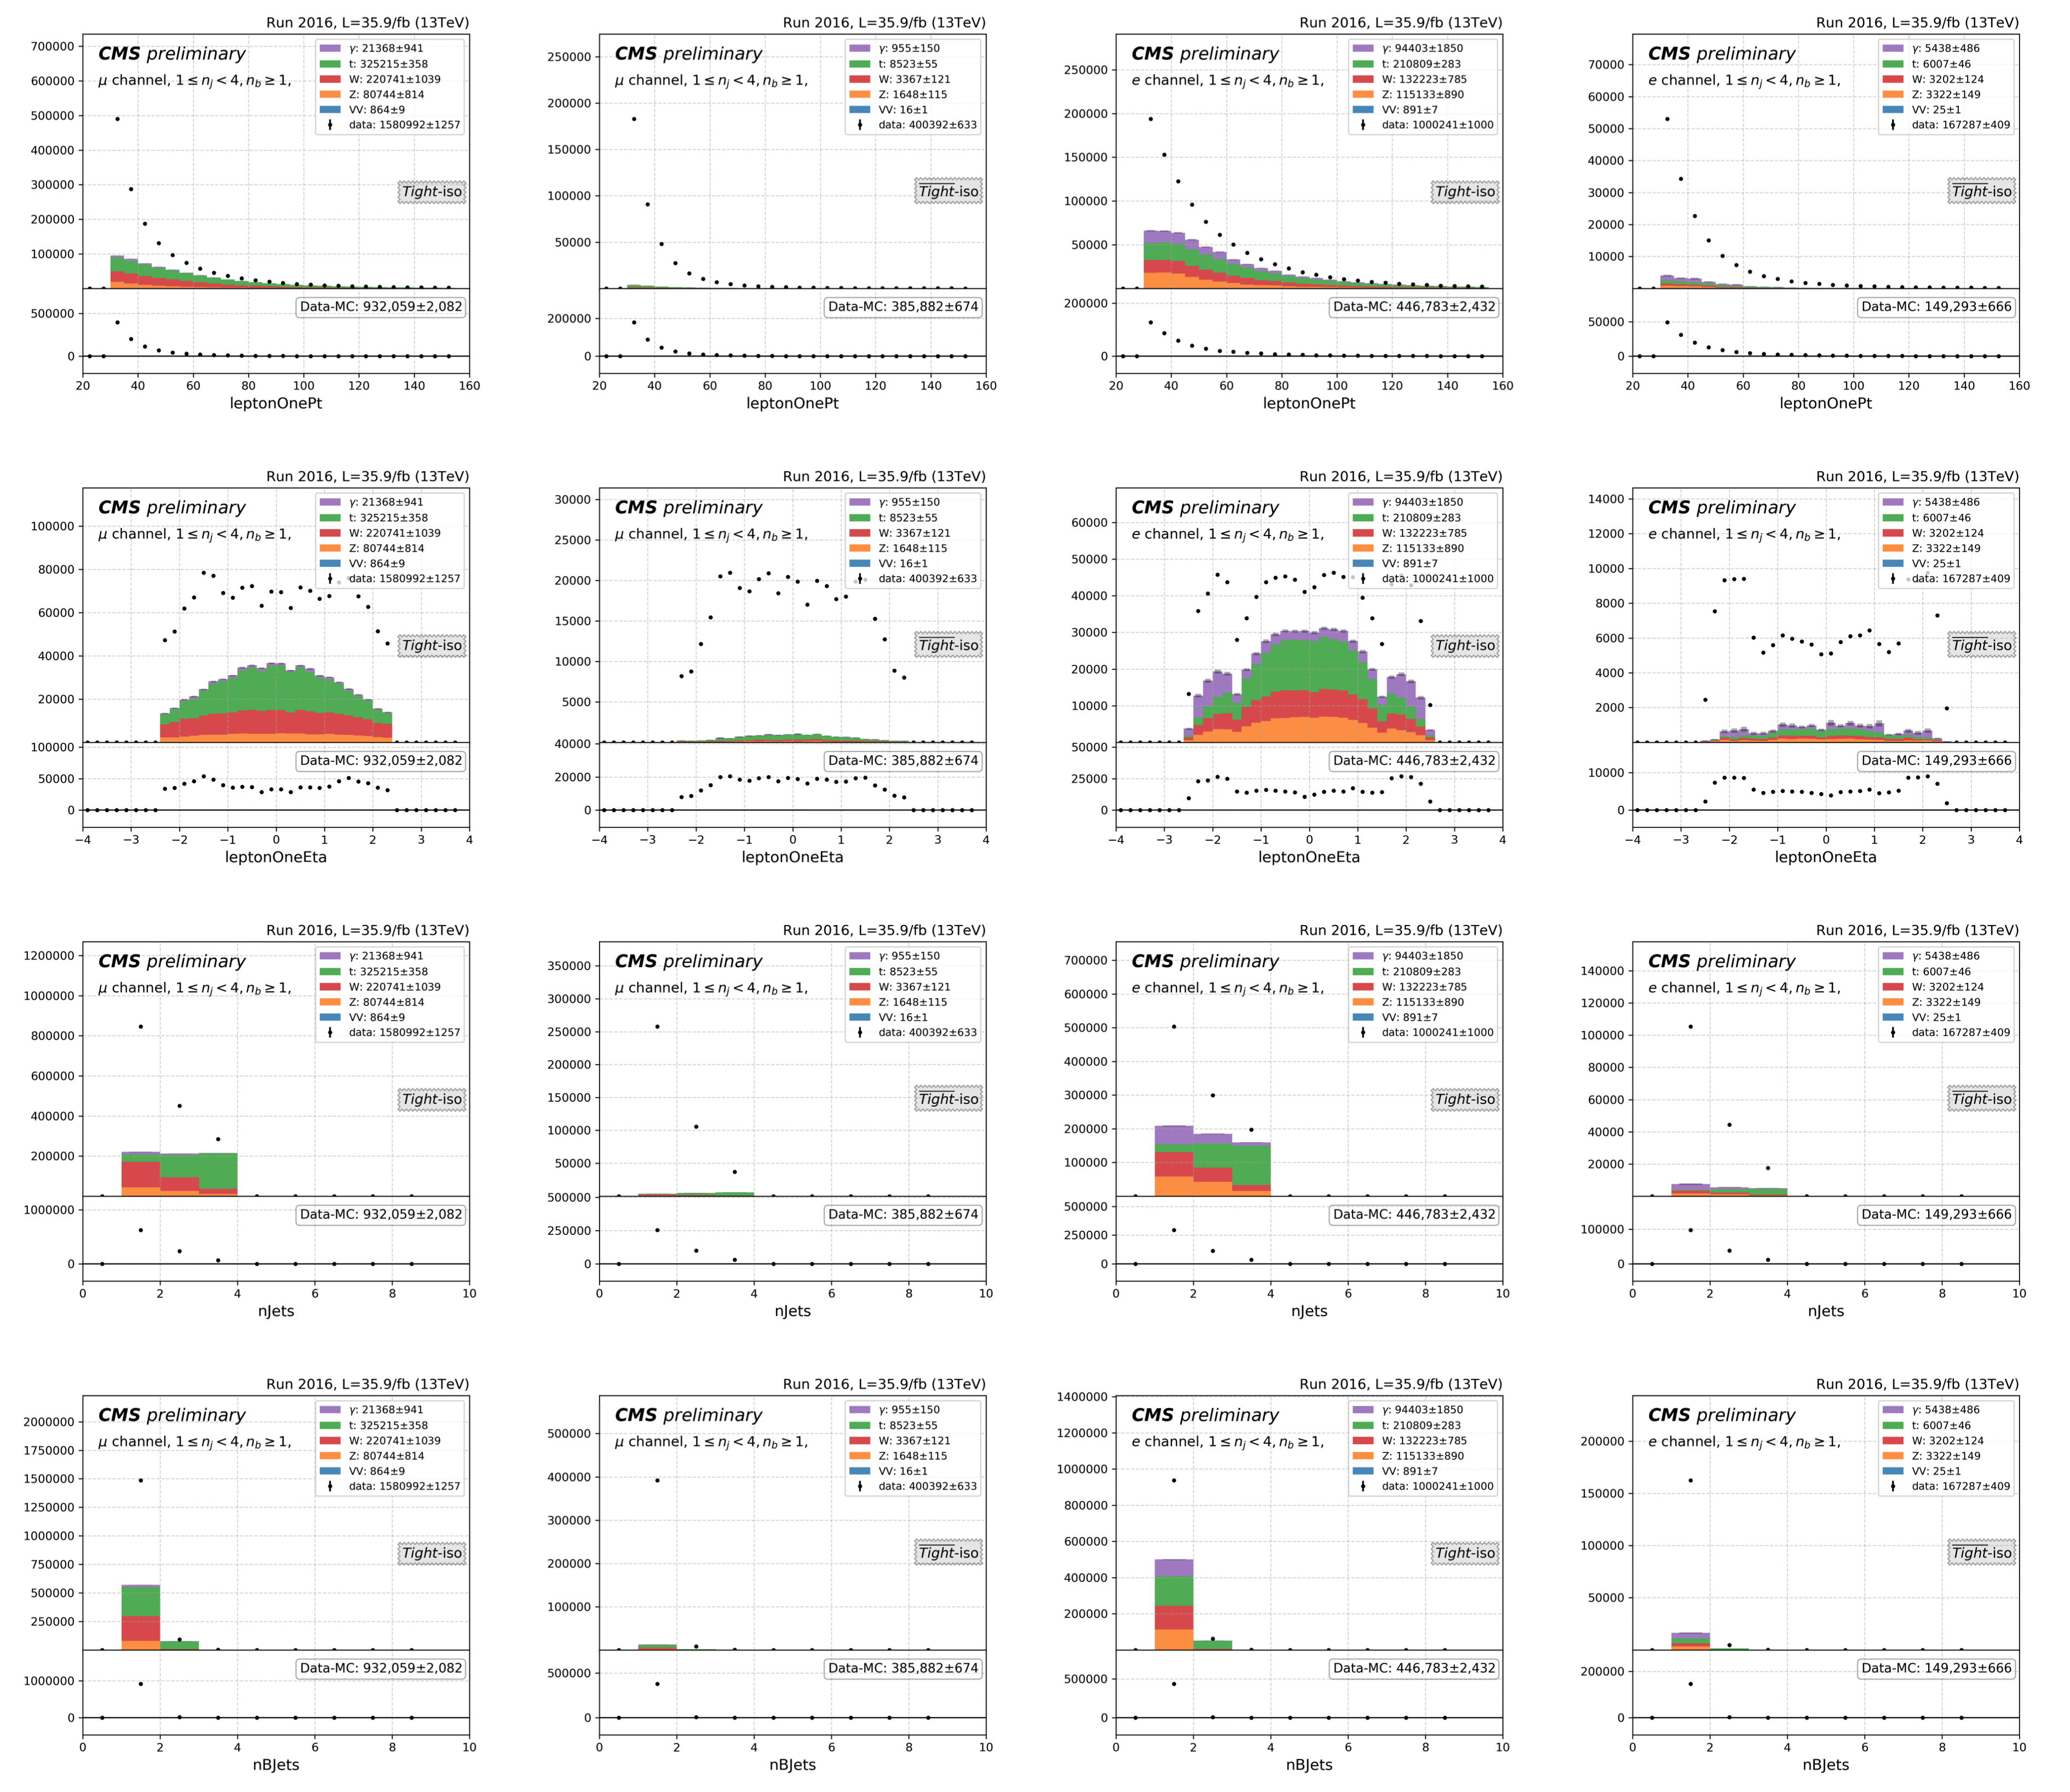
\includegraphics[width=0.99\textwidth]{chapters/Analysis/sectionBackground/figures/ljets_kinematics/123j1b.png}
    \caption{The iso and anti-iso region of $\mu$+jet (left two columns) and $e$+jet (right two columns) channel 
    with $1\leq n_j <4, n_b\geq1$, which is orthogonal to the $n_j\geq4,n_b\geq1$ signal region.}
    \label{fig:appendix:123j1b}
\end{figure}


\begin{figure}
    \centering
    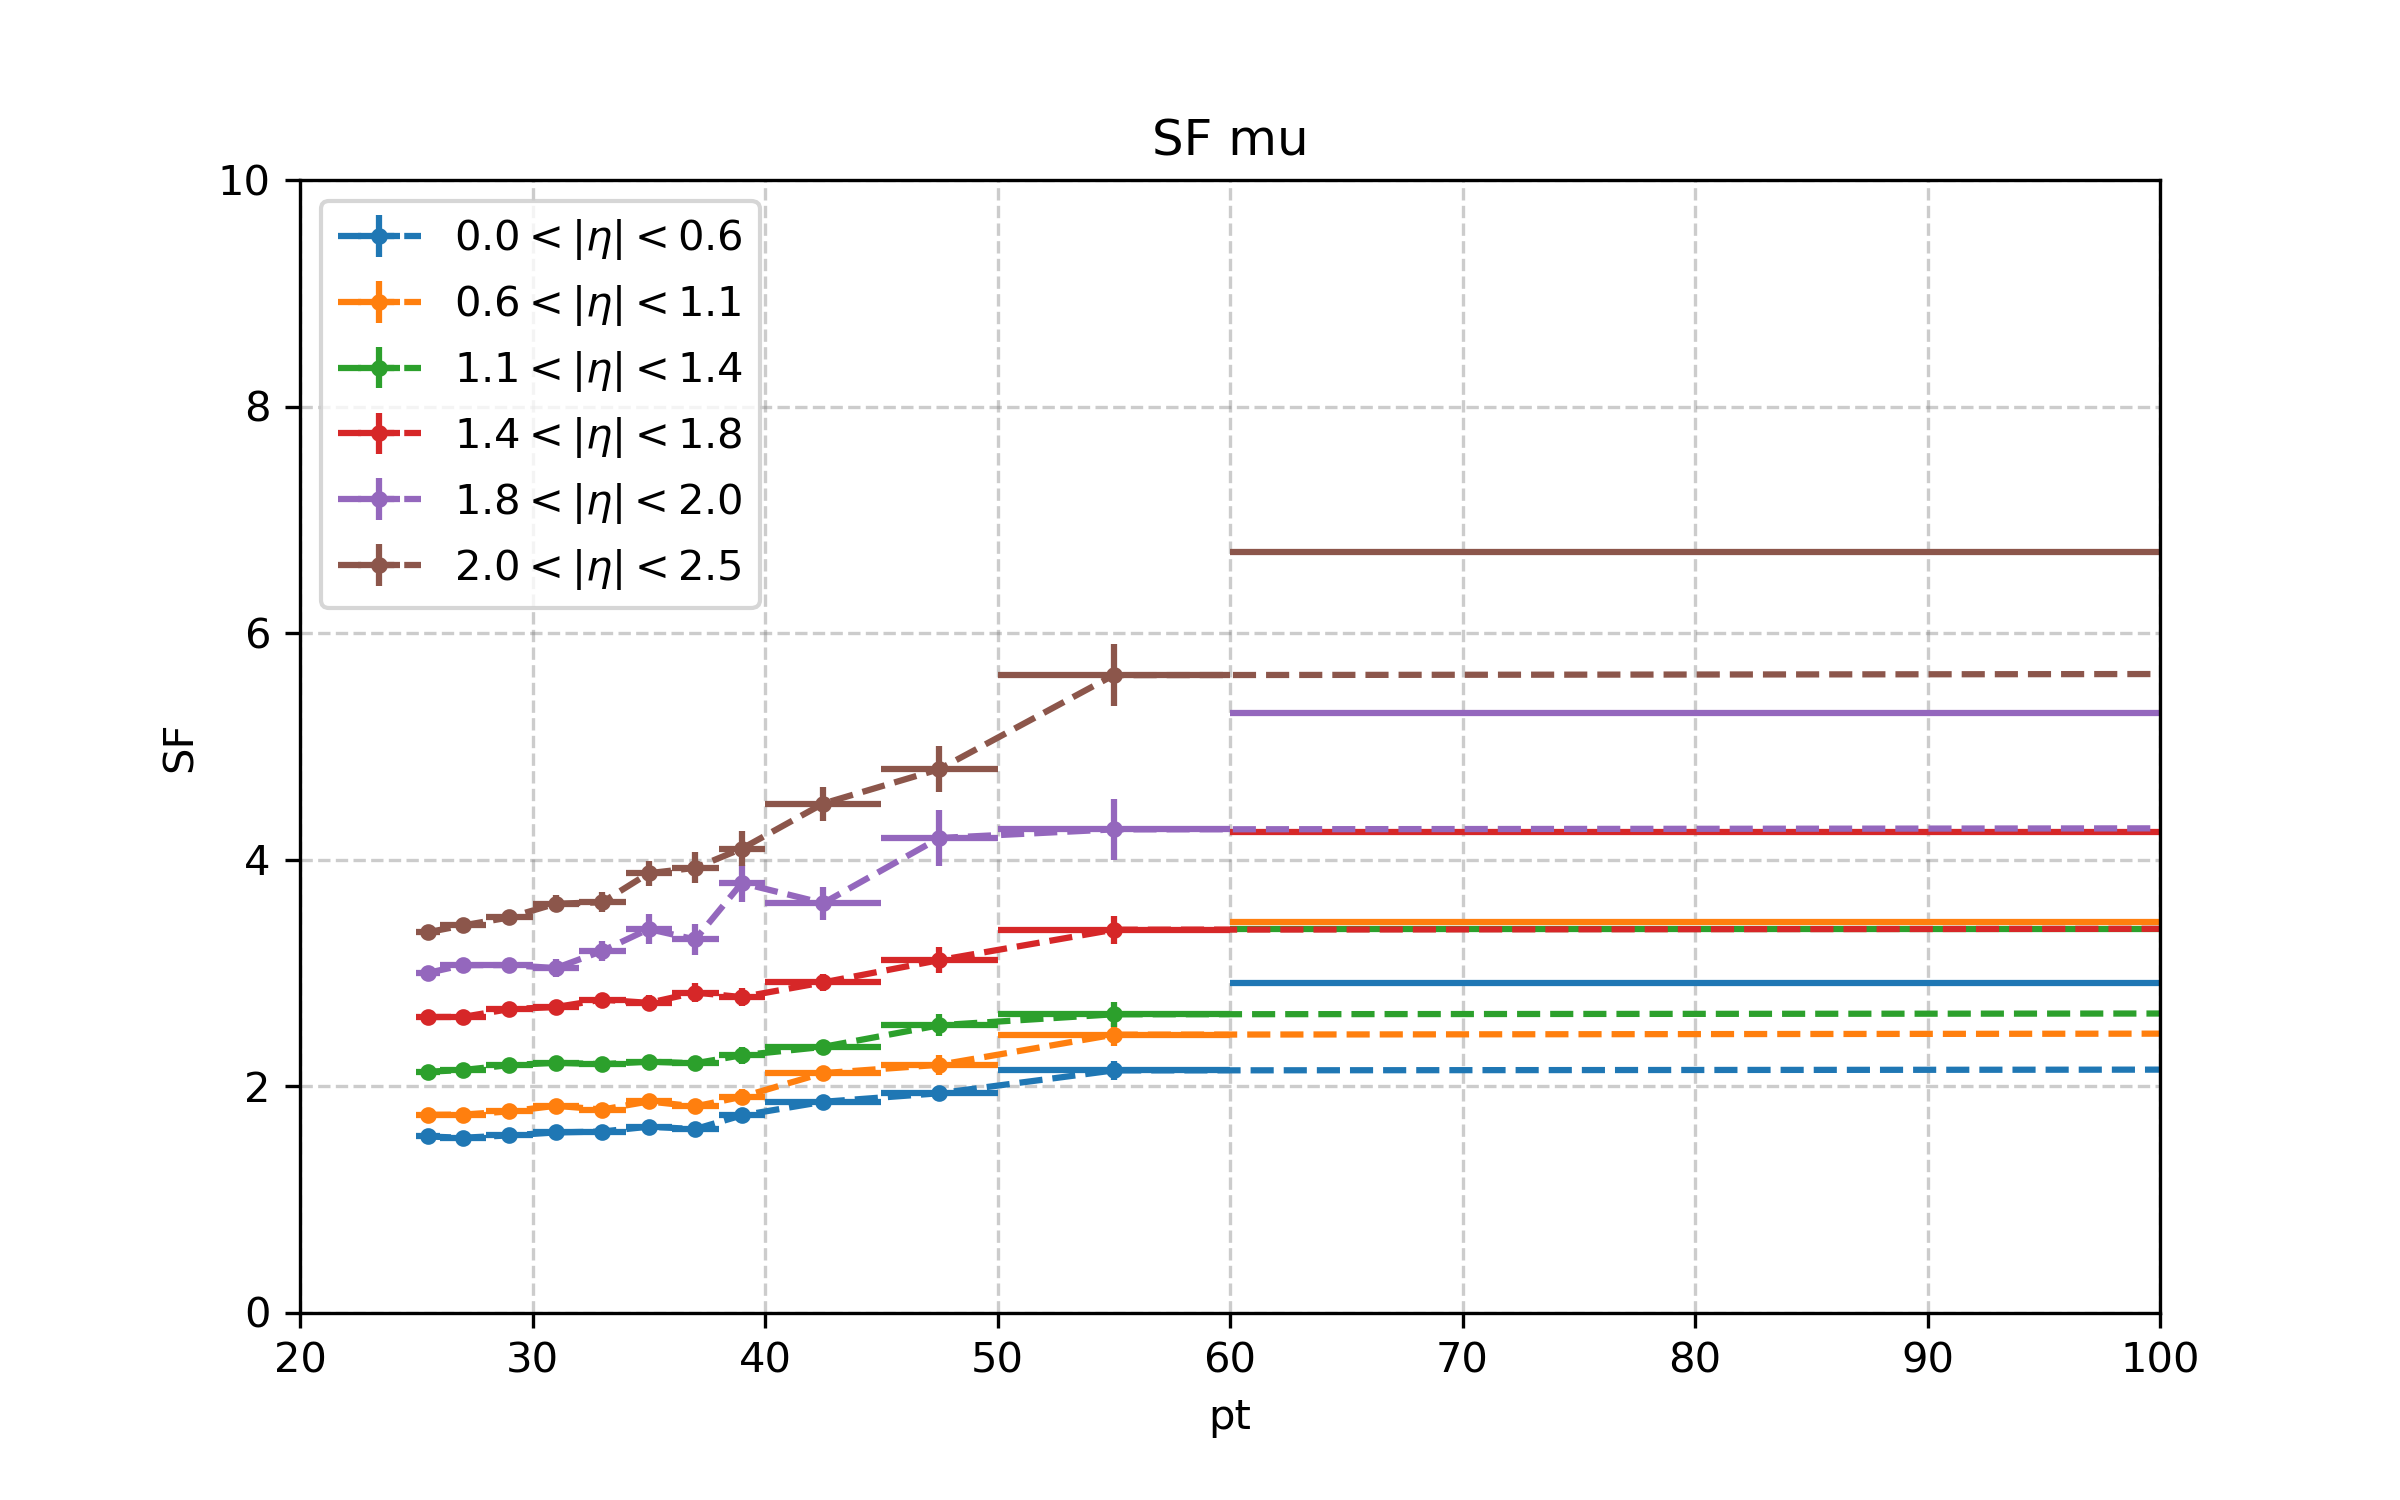
\includegraphics[width=0.49\textwidth]{chapters/Analysis/sectionBackground/figures/ljets_kinematics/123j1b/SF_mu_1d.png}
    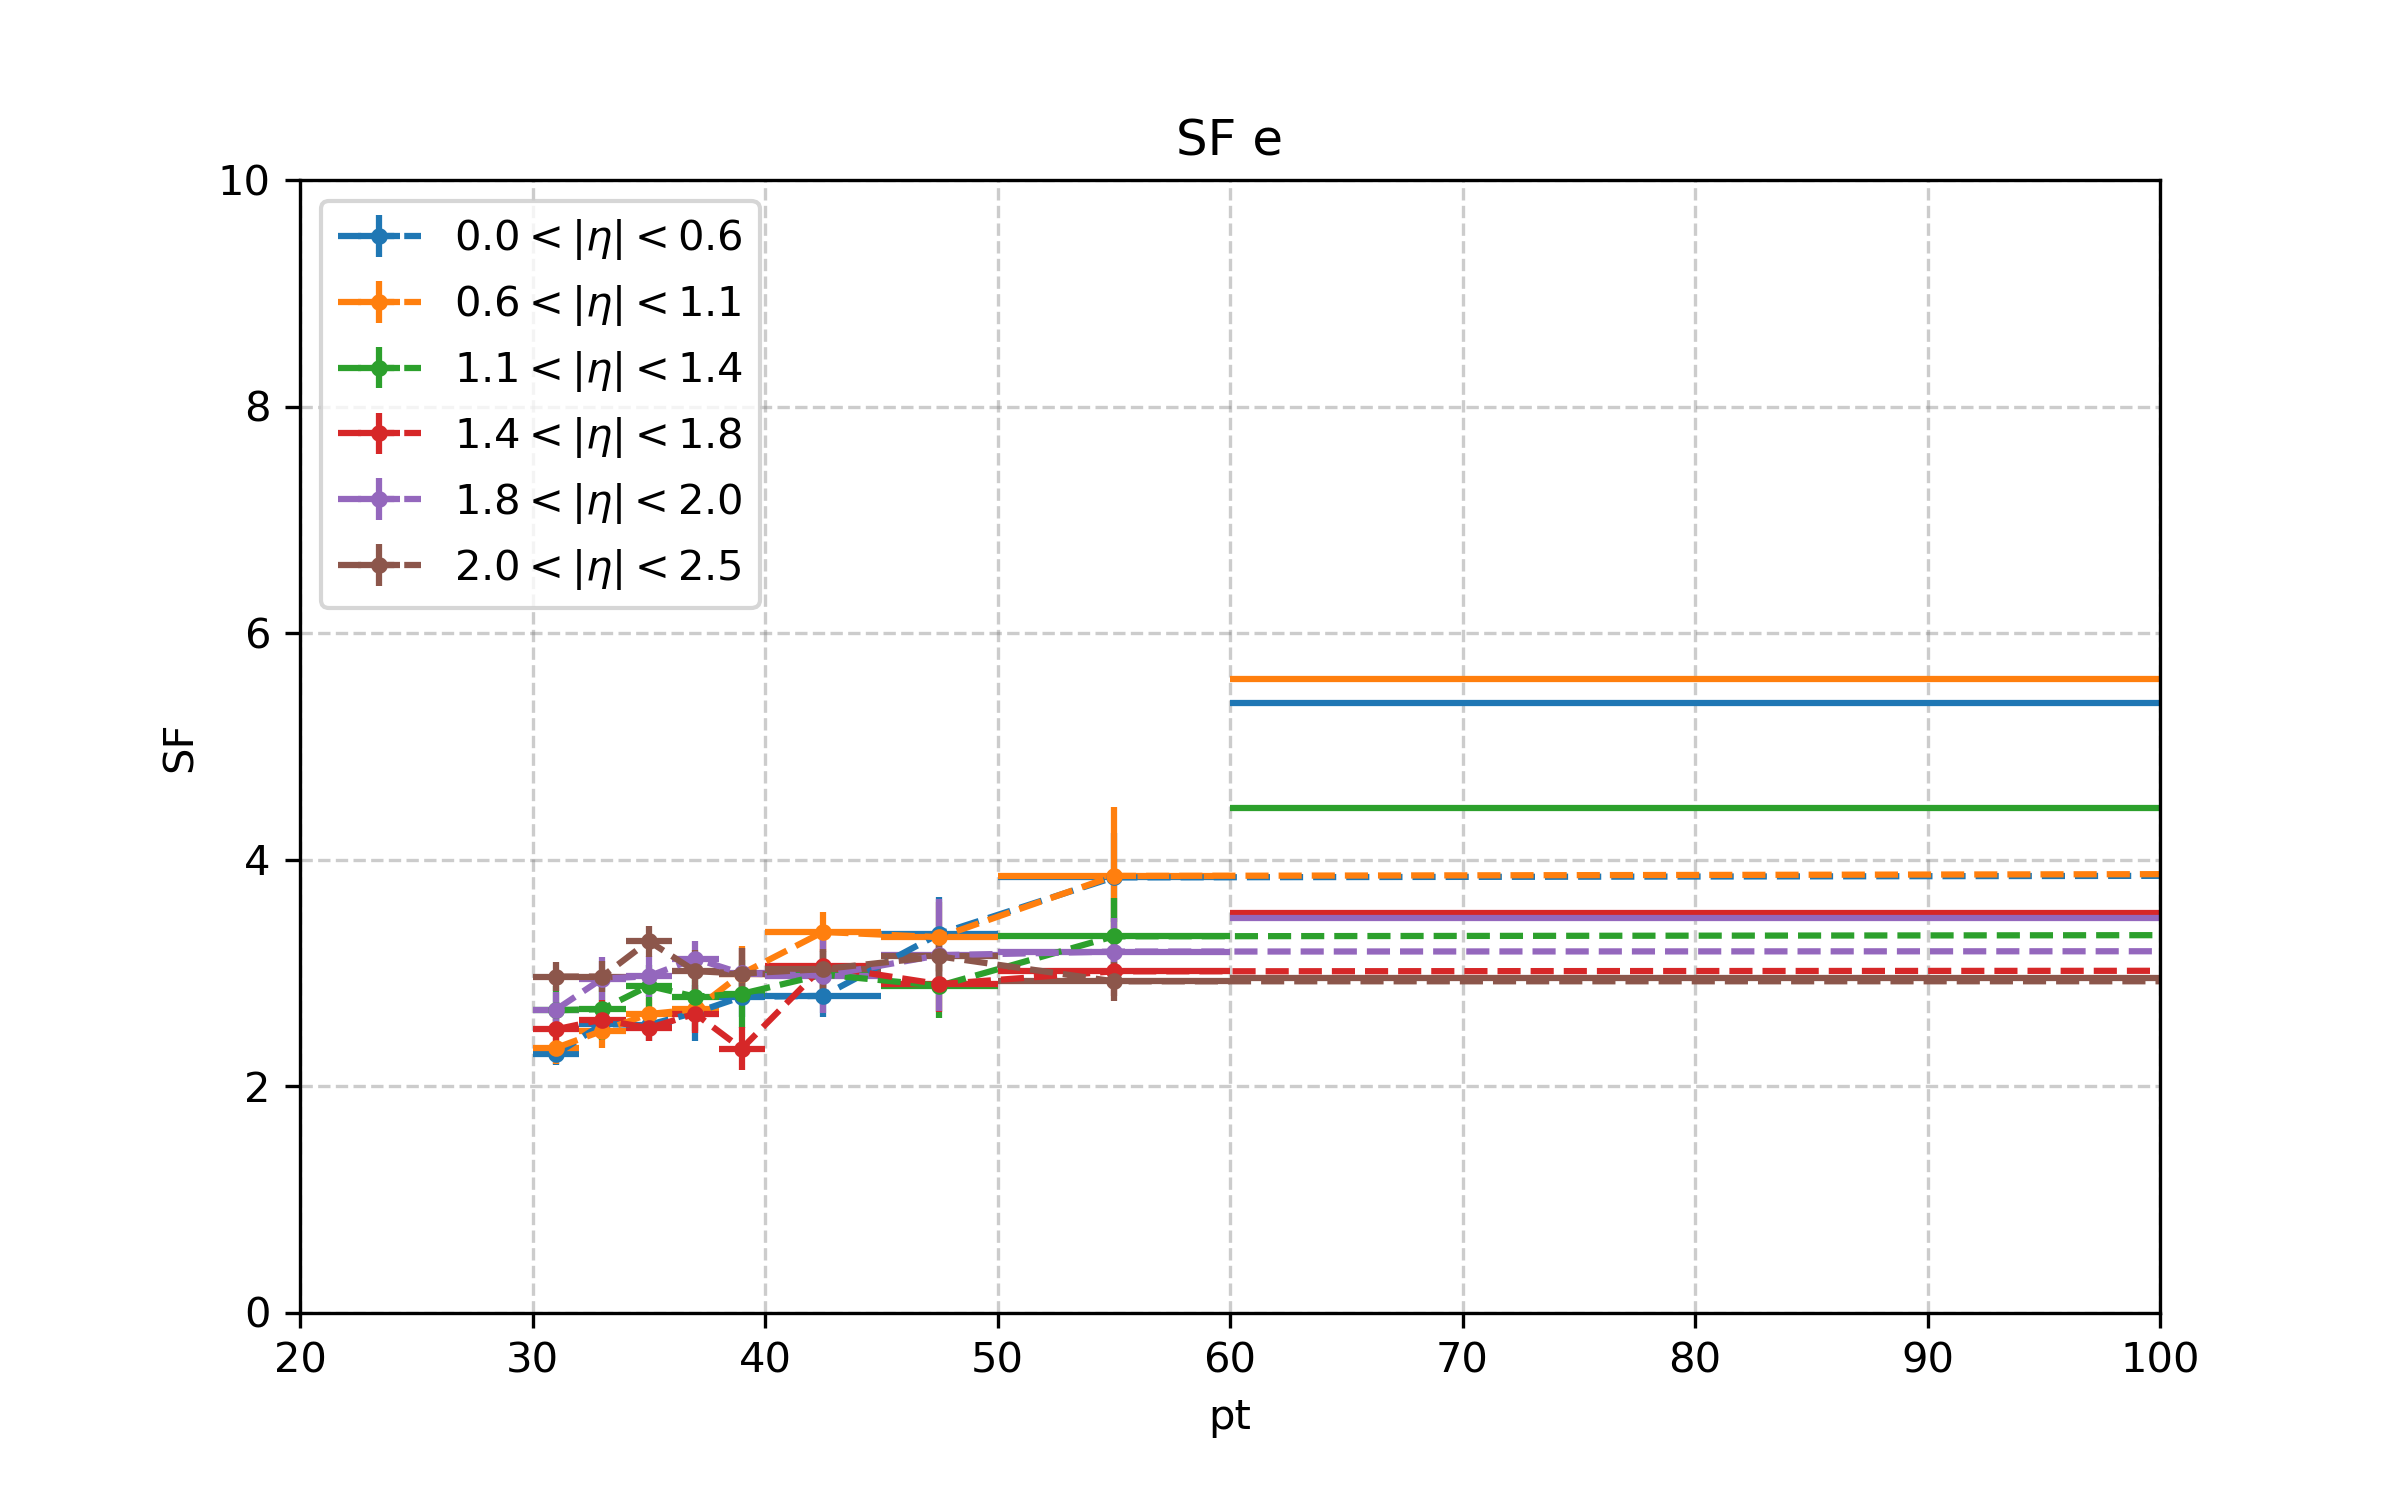
\includegraphics[width=0.49\textwidth]{chapters/Analysis/sectionBackground/figures/ljets_kinematics/123j1b/SF_e_1d.png}
    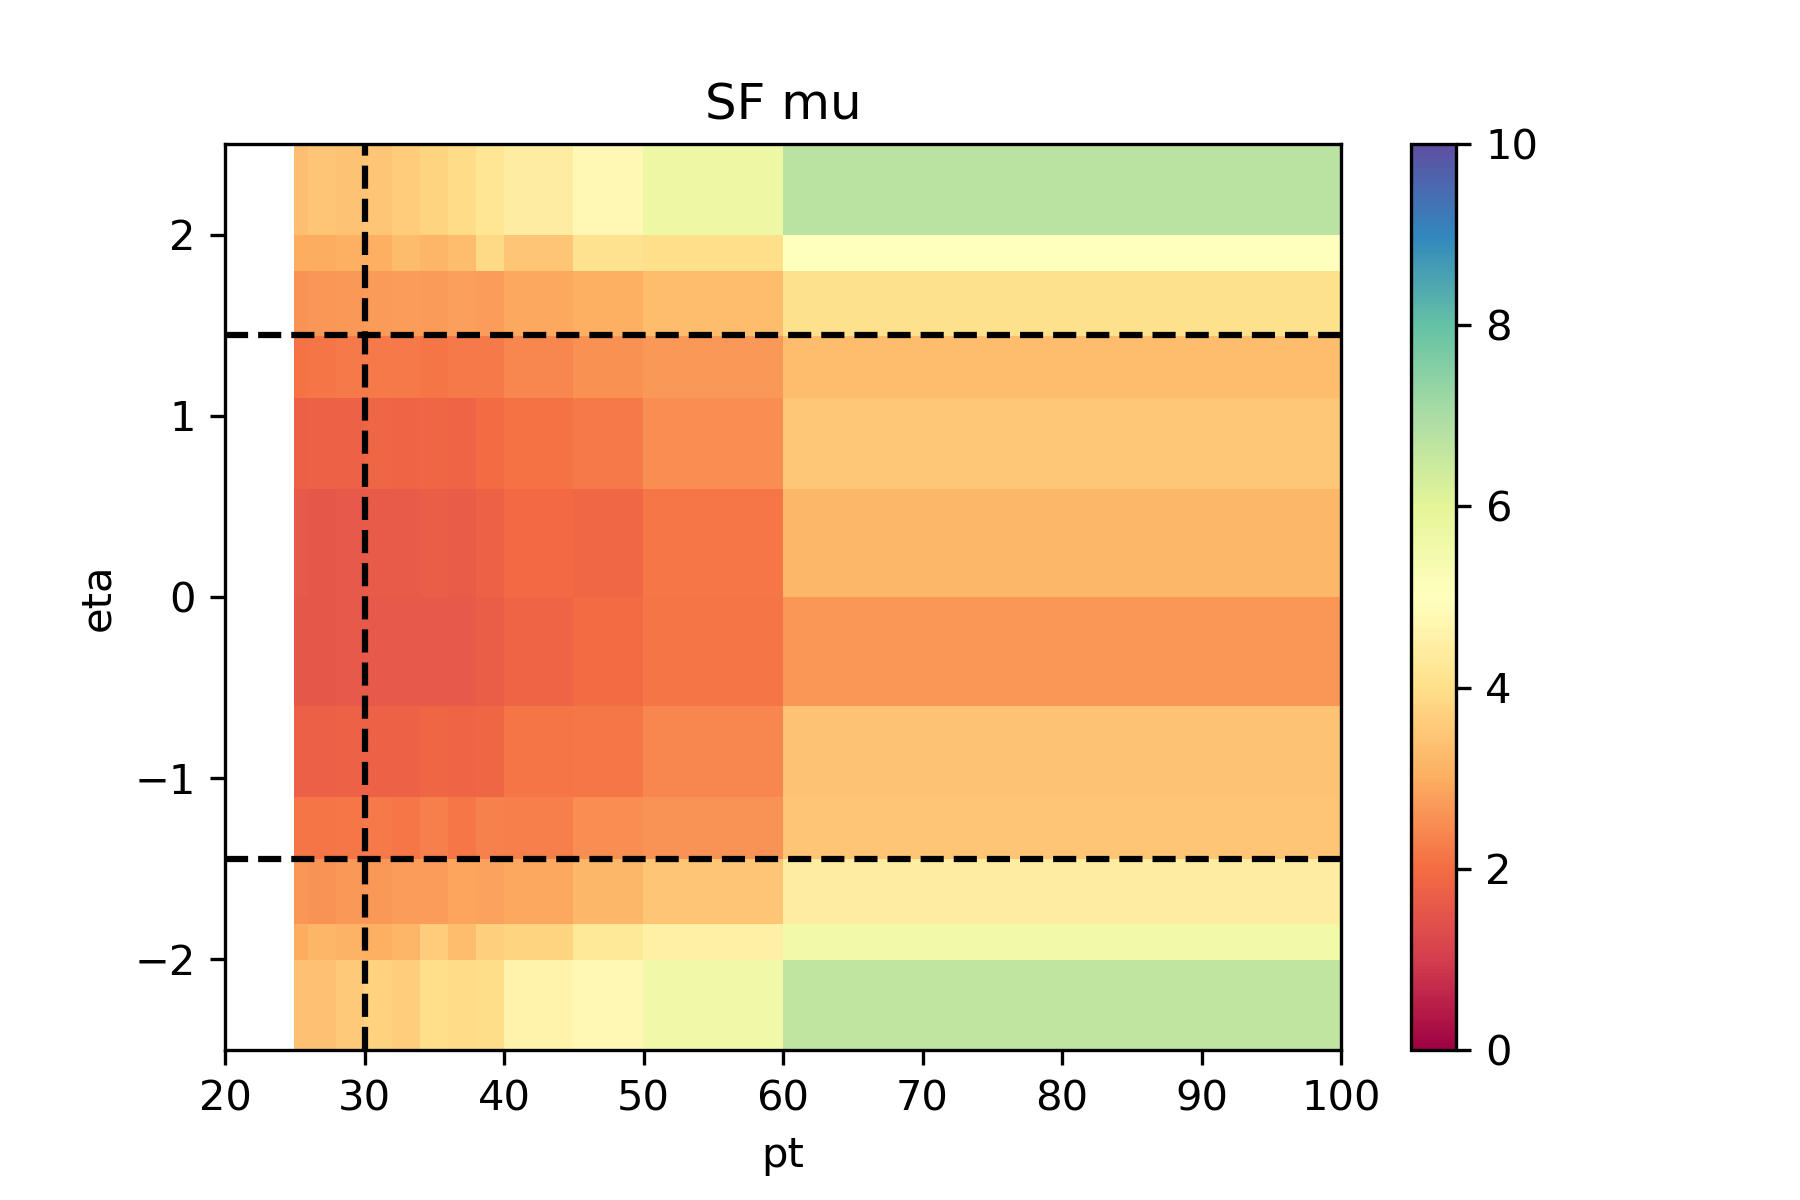
\includegraphics[width=0.49\textwidth]{chapters/Analysis/sectionBackground/figures/ljets_kinematics/123j1b/SF_mu_2d.png}
    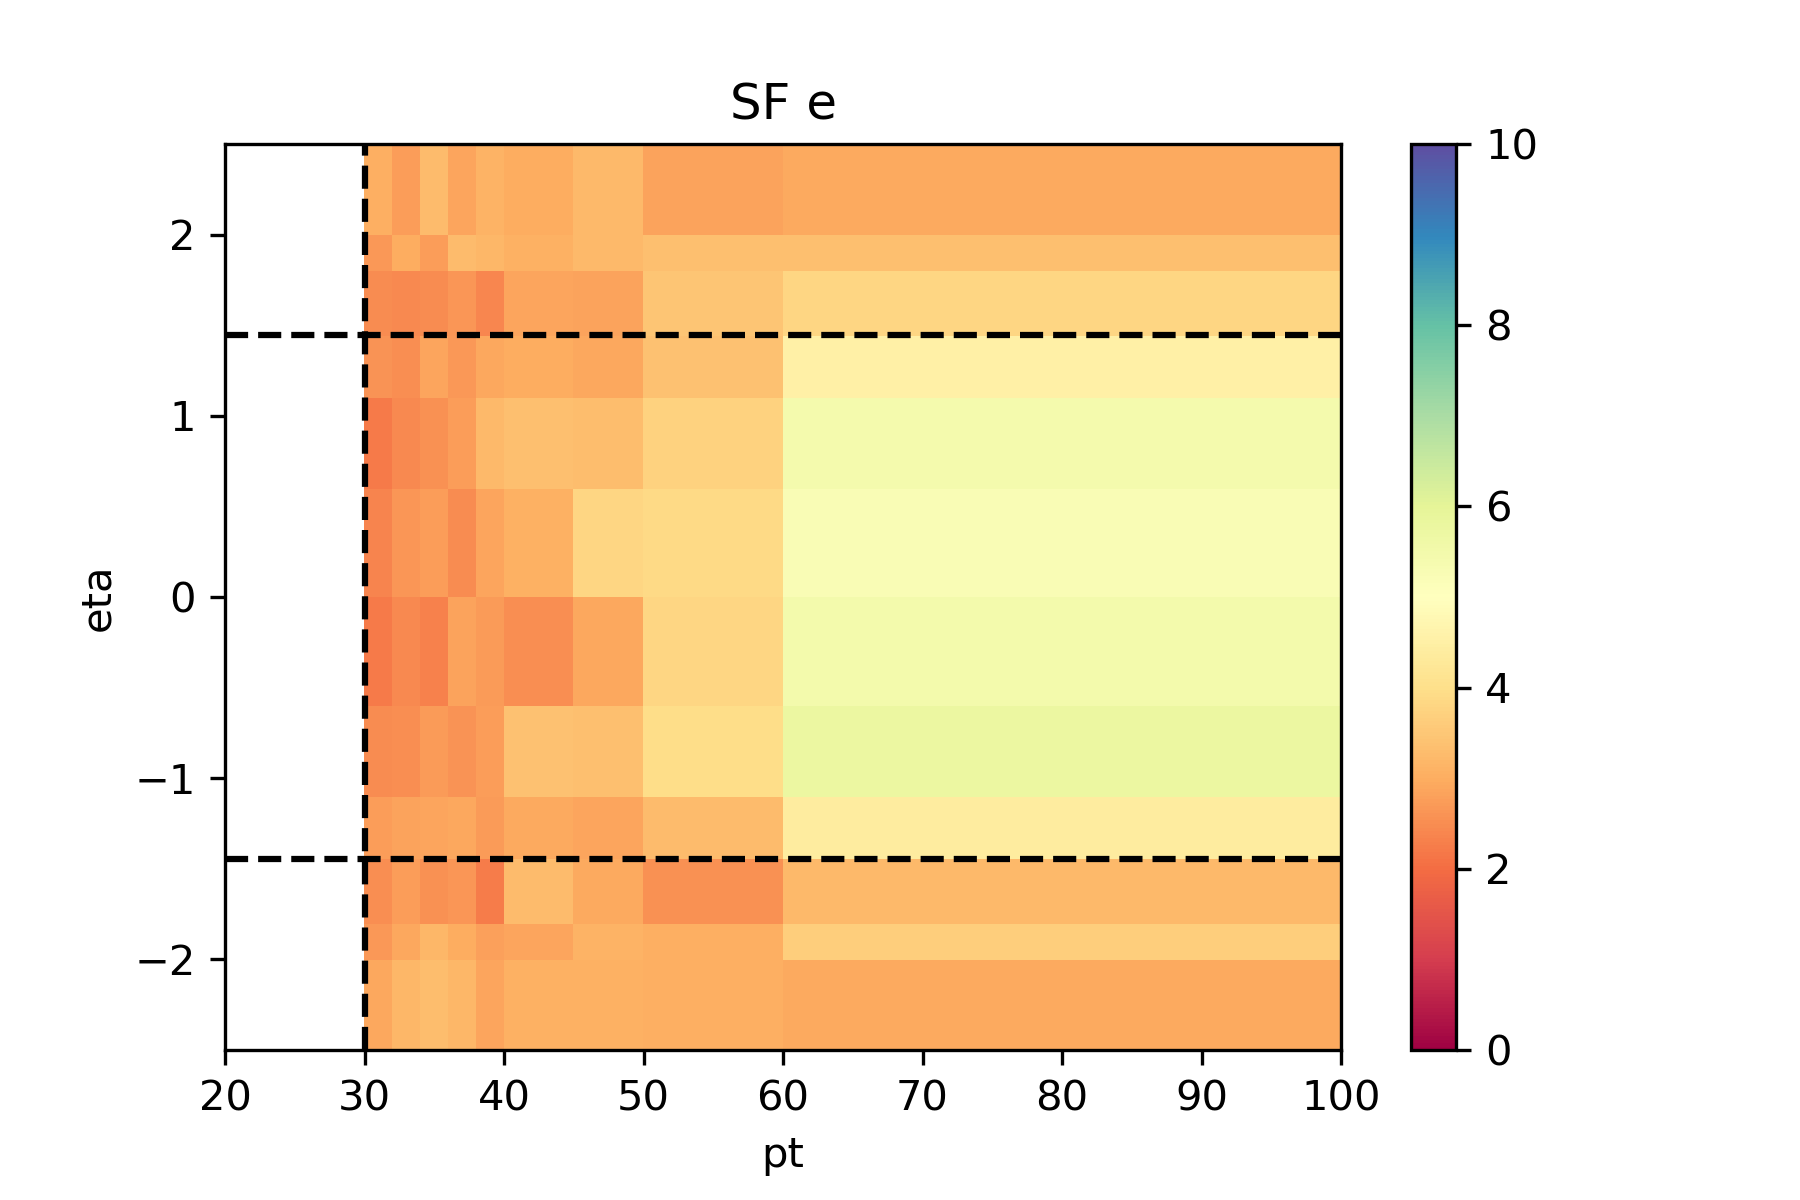
\includegraphics[width=0.49\textwidth]{chapters/Analysis/sectionBackground/figures/ljets_kinematics/123j1b/SF_e_2d.png}
    \caption{iso-to-antiiso SF in the $\mu$+jet (left) and $e$+jet (right) channel 
    with $1\leq n_j <4, n_b\geq1$ side-band region.}
    \label{fig:appendix:123j1b_sf}
\end{figure}



\begin{figure}
    \centering
    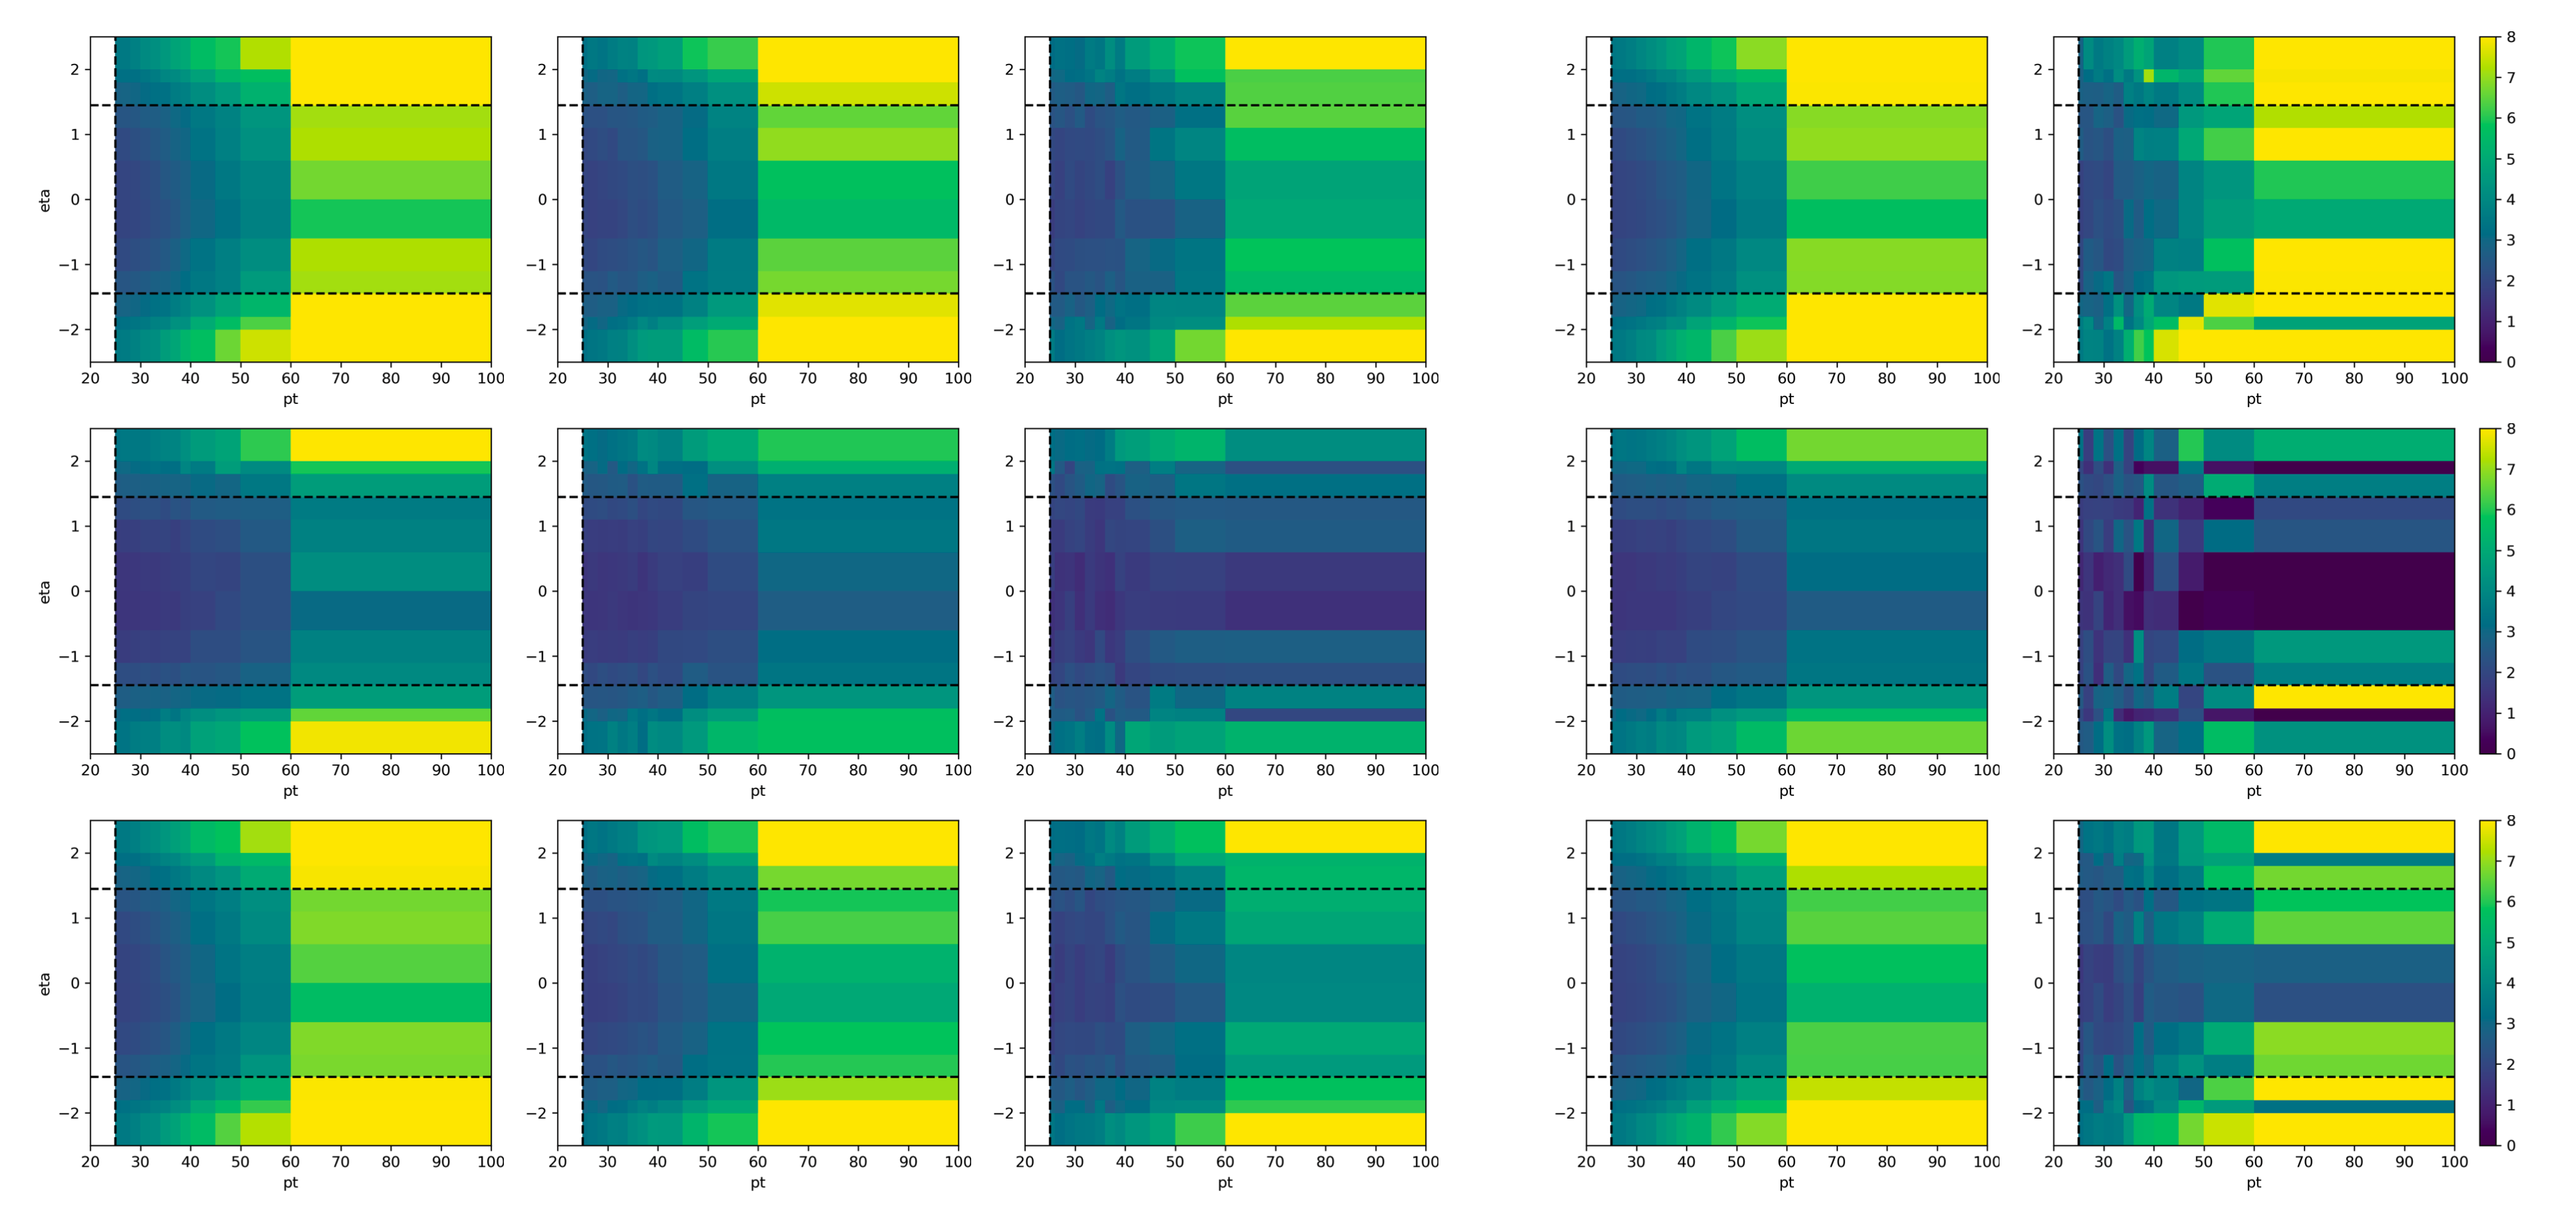
\includegraphics[width=0.99\textwidth]{chapters/Analysis/sectionBackground/figures/ljets_kinematics/sf_mu4j.png}
    \caption{iso-to-antiiso SF in the $\mu$+jet all regions.}
    \label{fig:appendix:allsf}
\end{figure}

\begin{figure}
    \centering
    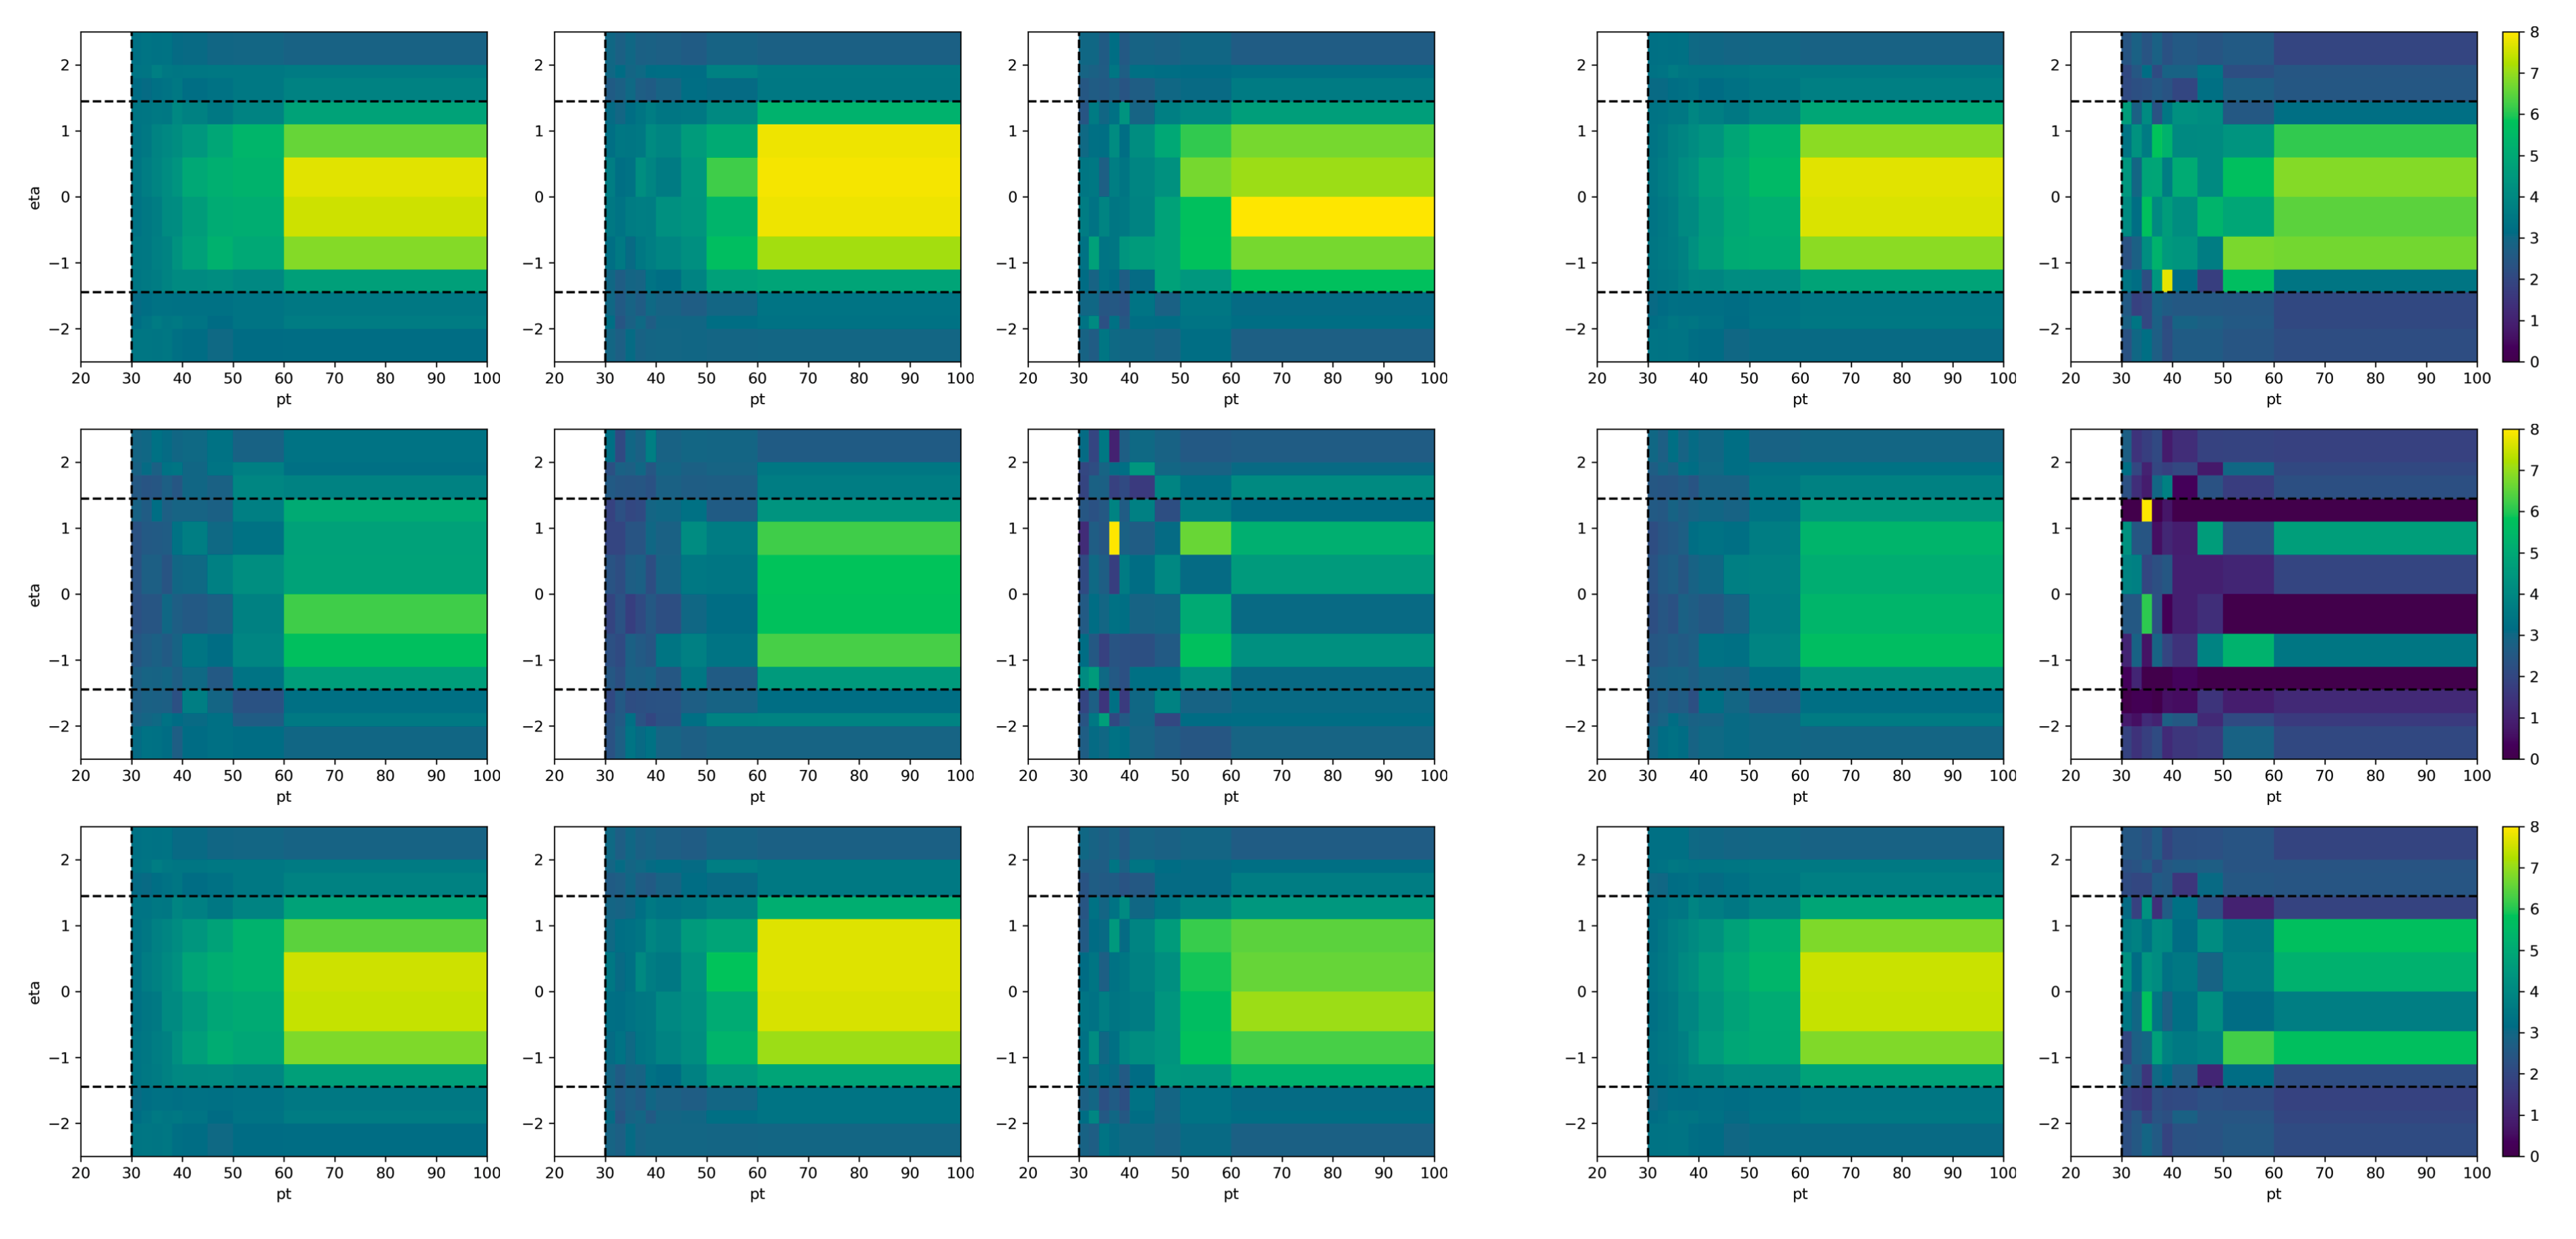
\includegraphics[width=0.99\textwidth]{chapters/Analysis/sectionBackground/figures/ljets_kinematics/sf_e4j.png}
    \caption{iso-to-antiiso SF in the $e$+jet all regions.}
    \label{fig:appendix:allsf}
\end{figure}




In the second approach, the HT-binned QCD MC is used. Figure~\ref{fig:appendix:4j1b} shows iso and antiiso region of $\mu$jet (left two columns) and $e$jet (right two columns) channel
with $n_j\geq4,n_b\geq1$ and the QCD MC in the signal region is shown as red line.

\begin{figure}
    \centering
    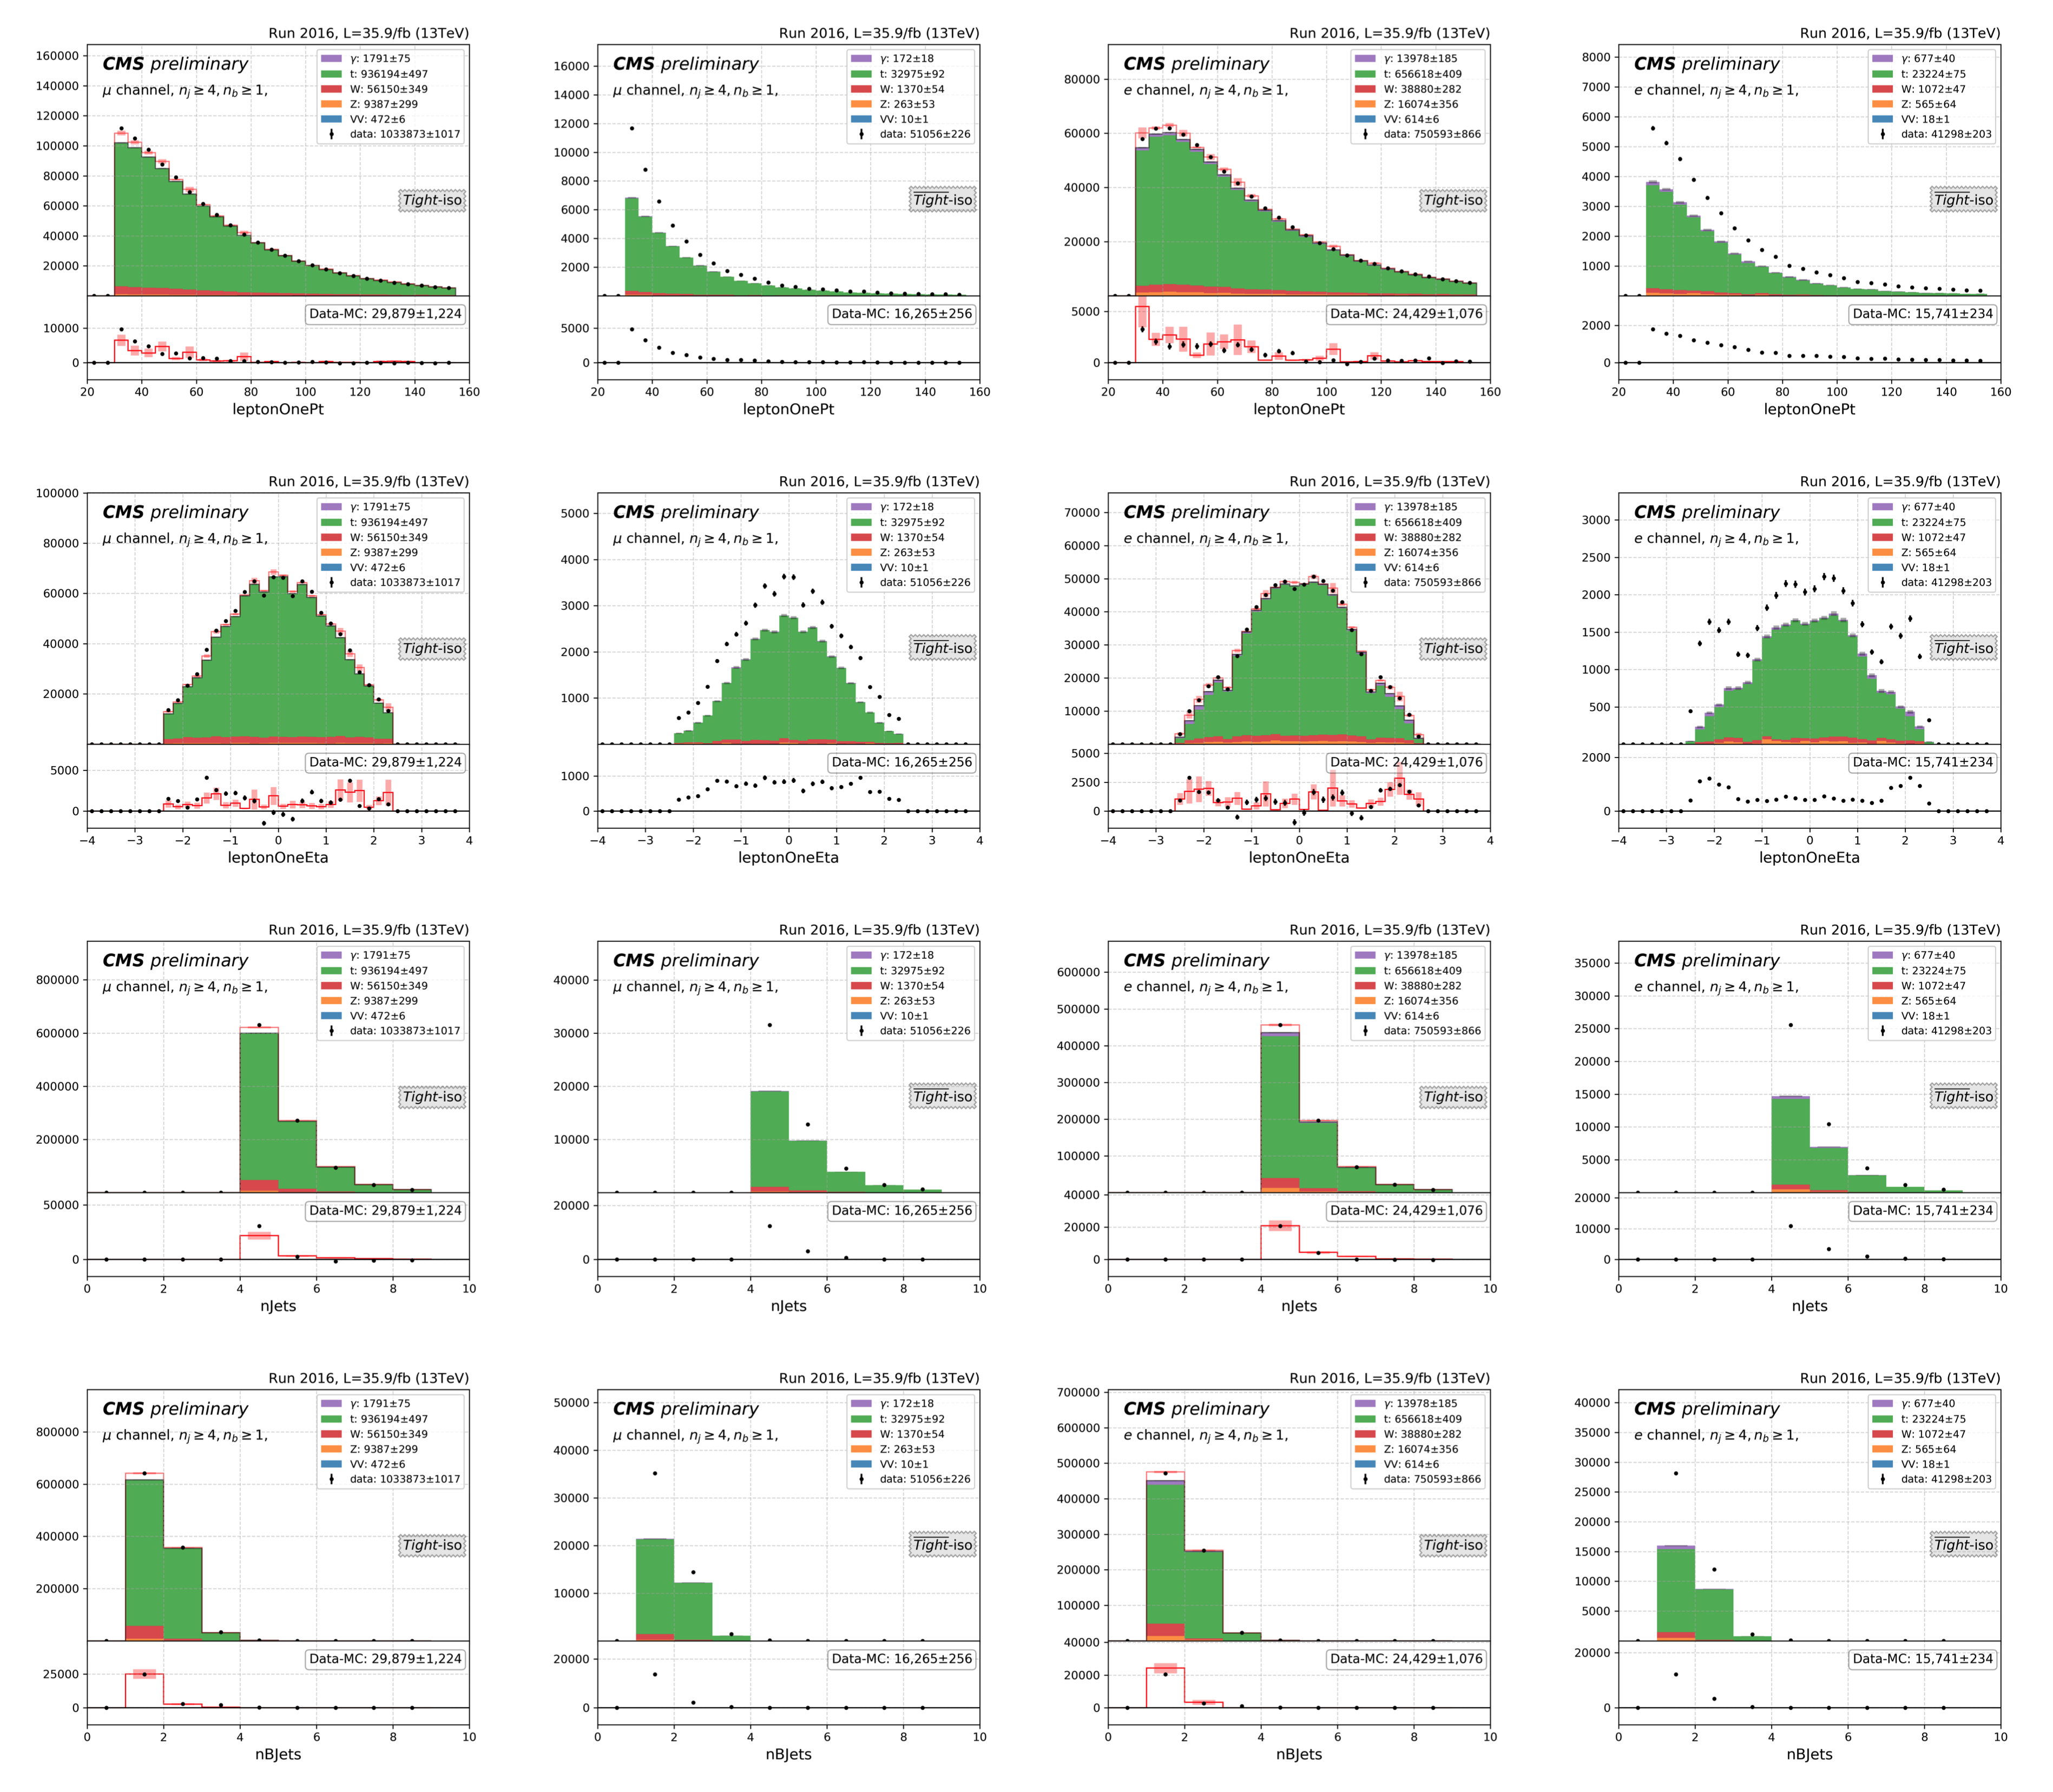
\includegraphics[width=0.99\textwidth]{chapters/Analysis/sectionBackground/figures/ljets_kinematics/4j1b.png}
    \caption{The iso and anti-iso region of $\mu$+jet (left two columns) and $e$+jet (right two columns) channel 
    with $n_j\geq4,n_b\geq1$, the signal region.}
    \label{fig:appendix:4j1b}
\end{figure}




\begin{figure}
    \centering
    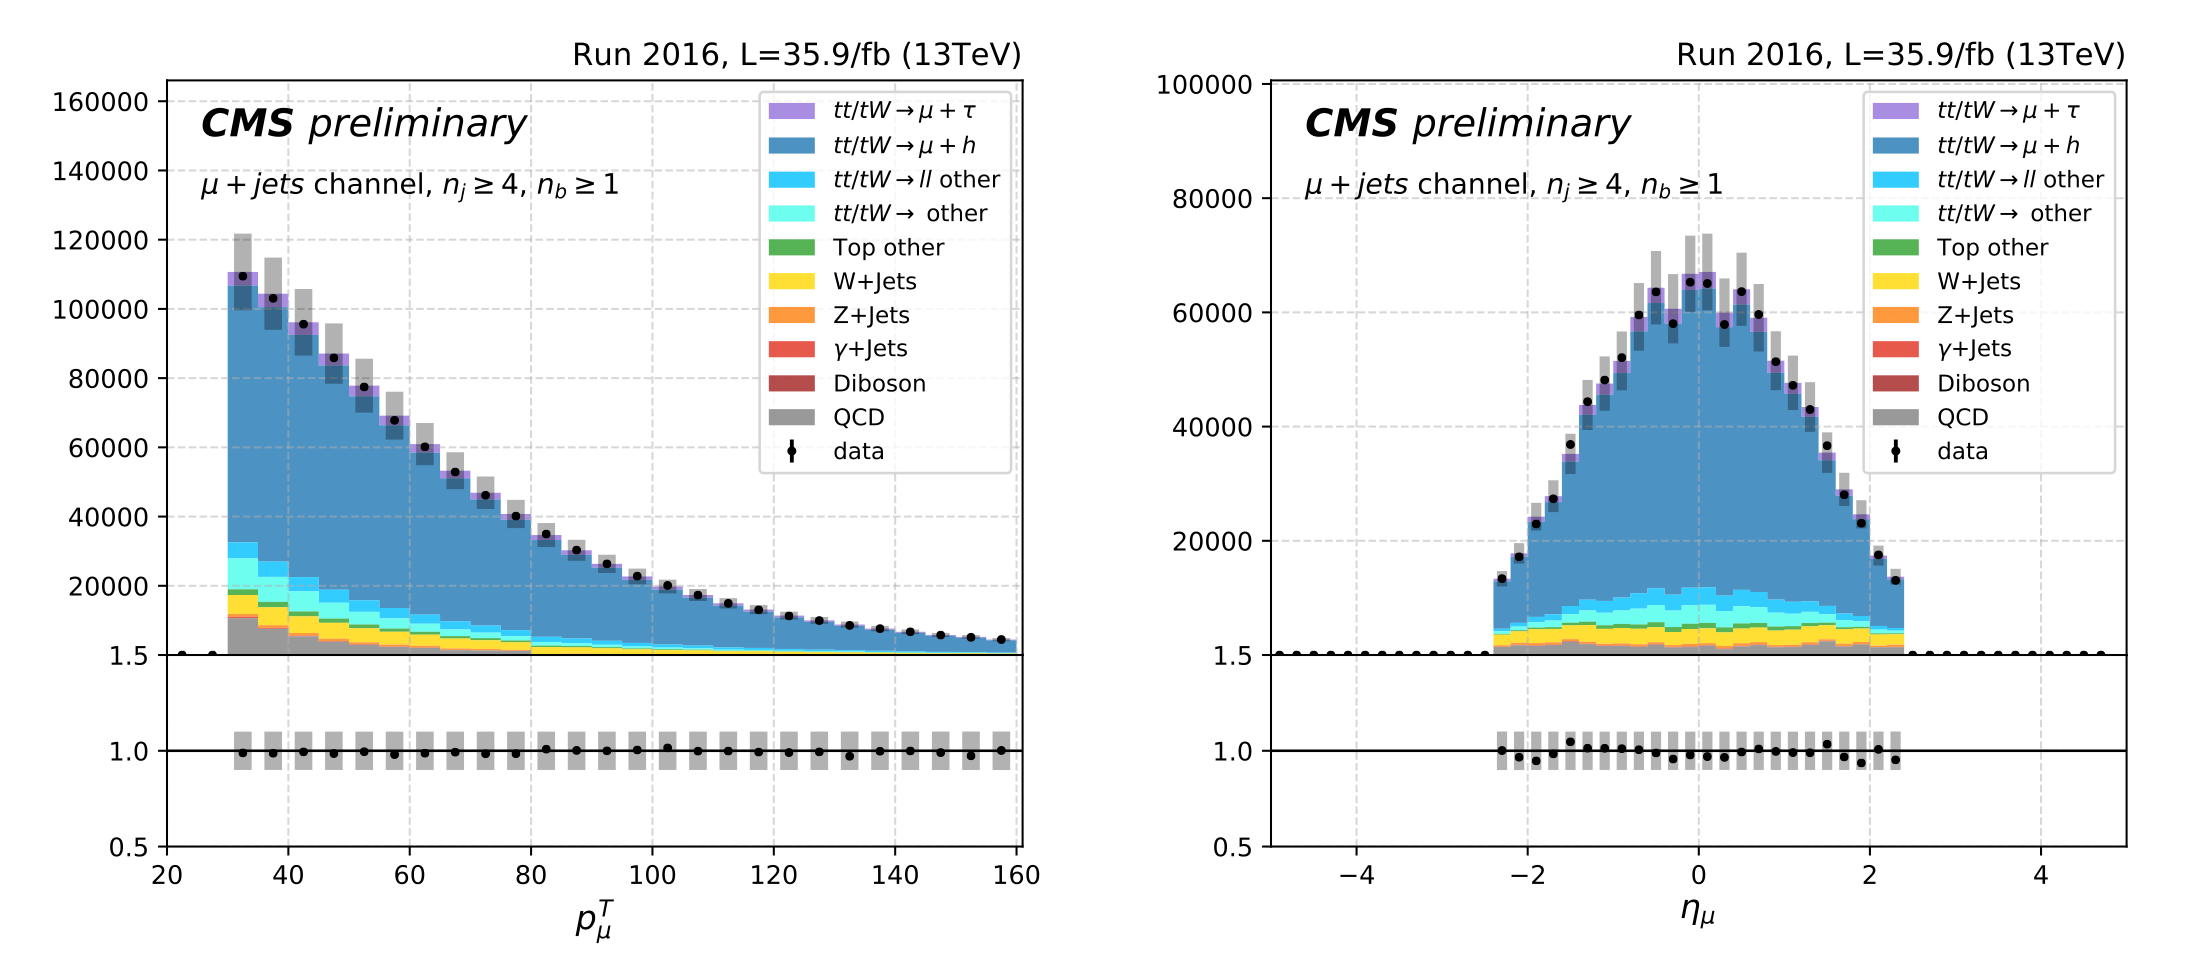
\includegraphics[width=0.99\textwidth]{chapters/Analysis/sectionBackground/figures/ljets_application/ddNorm_ddShape_mu4j.png}
    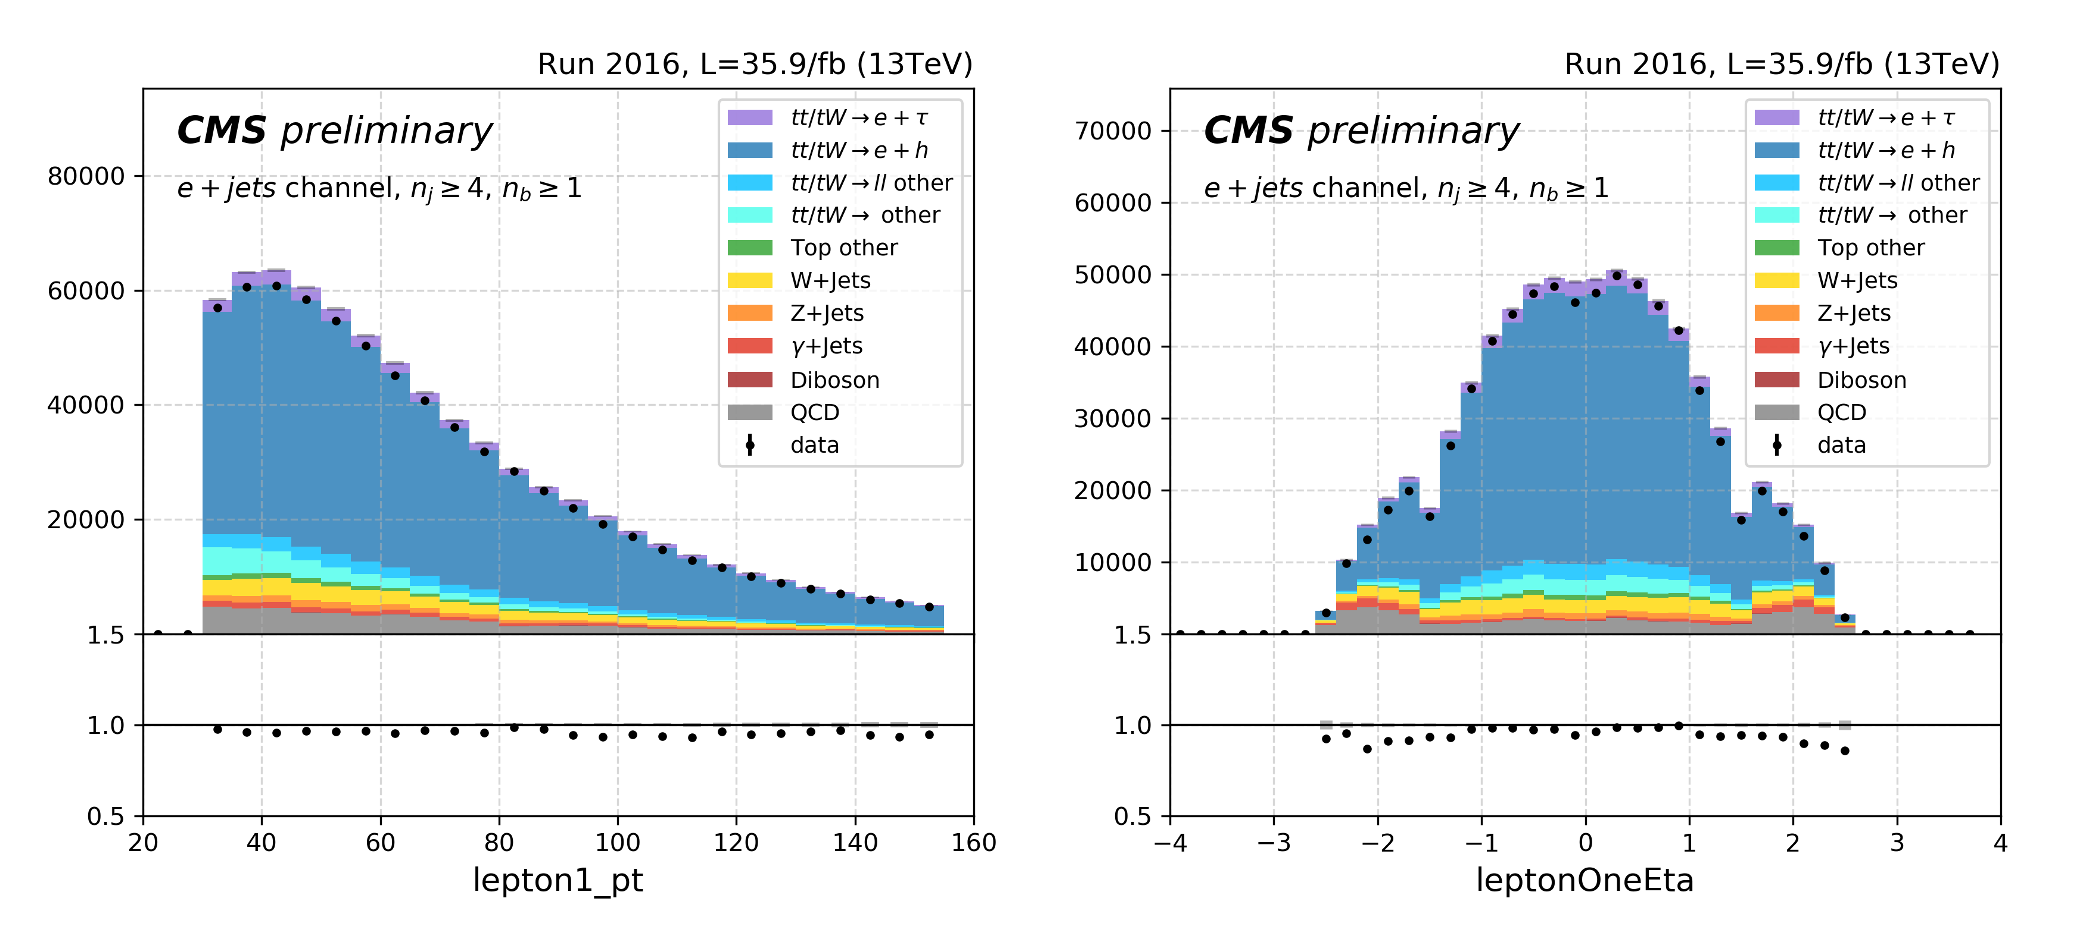
\includegraphics[width=0.99\textwidth]{chapters/Analysis/sectionBackground/figures/ljets_application/ddNorm_ddShape_e4j.png}
    \caption{Fully data-driven QCD estimation.}
    \label{fig:app:QCD:application_SFNorm_ddShape}
\end{figure}

\begin{figure}
    \centering
    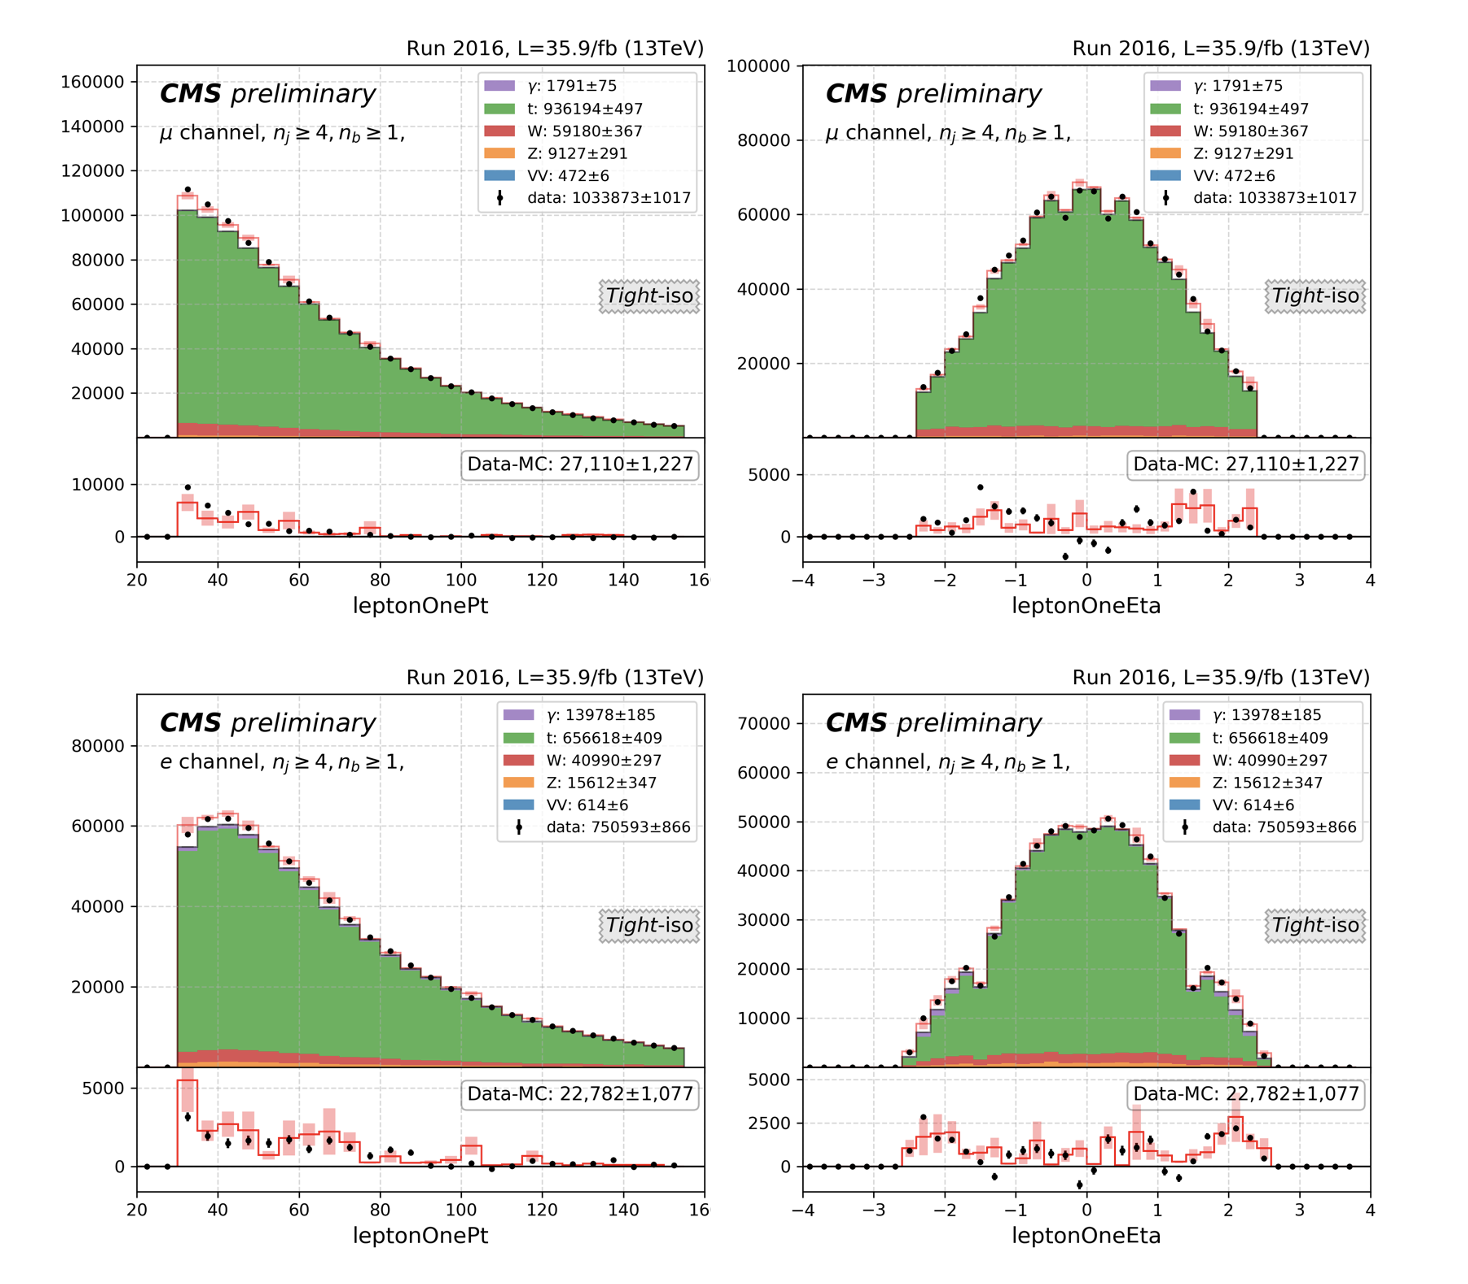
\includegraphics[width=0.99\textwidth]{chapters/Analysis/sectionBackground/figures/ljets_application/mcNorm_mcShape.png}
    \caption{Fully MC-based QCD estimation}
    \label{fig:app:QCD:application_mc}
\end{figure}

\begin{figure}
    \centering
    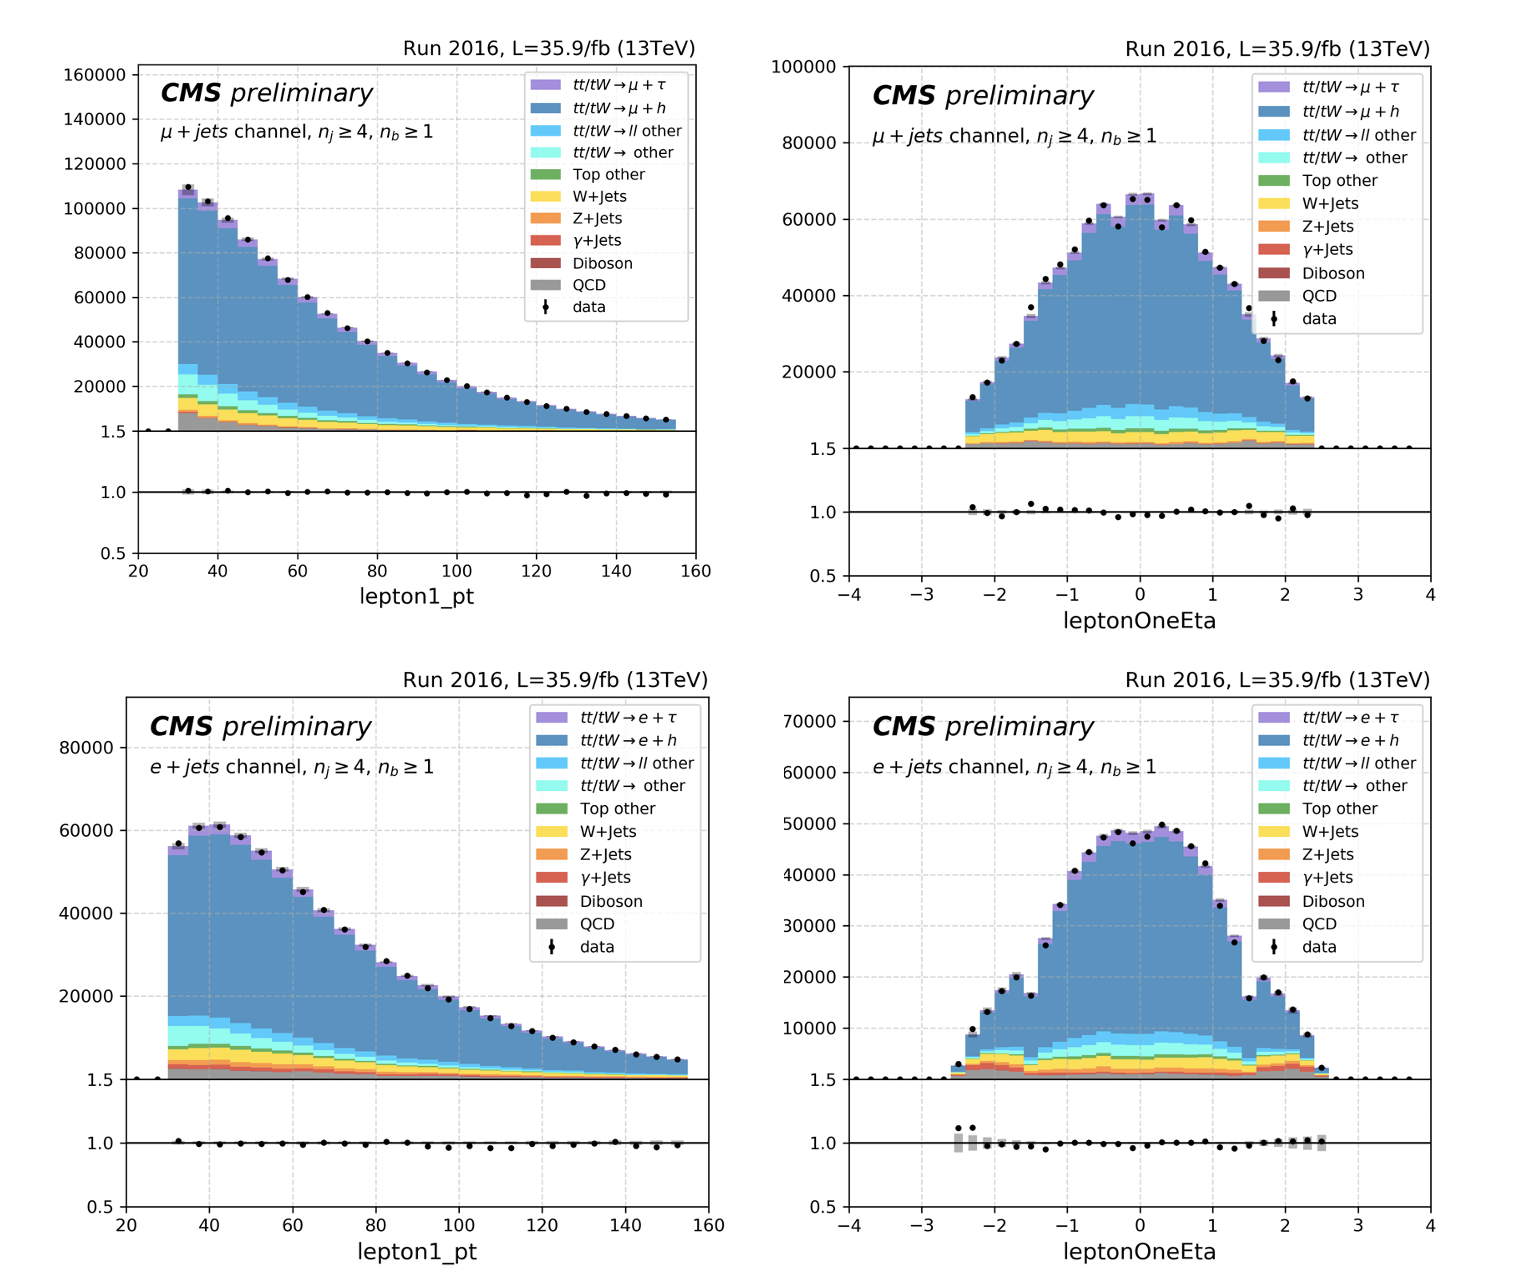
\includegraphics[width=0.99\textwidth]{chapters/Analysis/sectionBackground/figures/ljets_application/mcNorm_ddShape.png}
    \caption{Data-driven shape normalized by MC-based normalization.}
    \label{fig:app:QCD:application_mcNorm_ddShape}
\end{figure}
\FloatBarrier


\FloatBarrier



\subsection{Same-sign estimate}

This estimation relies on the dearth of standard model processes that can give rise to same-sign lepton pairs.  Because of this it is expected that most events with same-sign lepton pairs are the result of at least on of the leptons not being the result of a prompt bosonic decay, but are produced by a hadronic jet.  It is further assumed that this process will give rise to misidentifying hadronic jets as leptons in near equal measure between the same sign and opposite sign selections.  This is verified by deriving a scale factor in an isolation inverted region.

The process of deriving the estimate is simple enough: all the same selection requirements that are applied in the nominal analysis selection are applied to the side-band region with the exception of the opposite sign requirement, which is inverted.  The same is done for all of the relevant MC samples in order to determine what component of the same-sign data sample will already be estimated by the MC.  Finally, a correction factor is applied to account for any difference in the probability of the QCD giving rise to opposite sign and same sign final states.

To verify the method, a control region enriched in $\PZ\to\tau\tau$ is examined for the $\mu\tau$ and $e\tau$ final states.  A comparison of data and simulation in both the same sign and opposite sign regions are shown in figure~\ref{fig:ltau_fakes}.

\begin{figure}
    \centering
    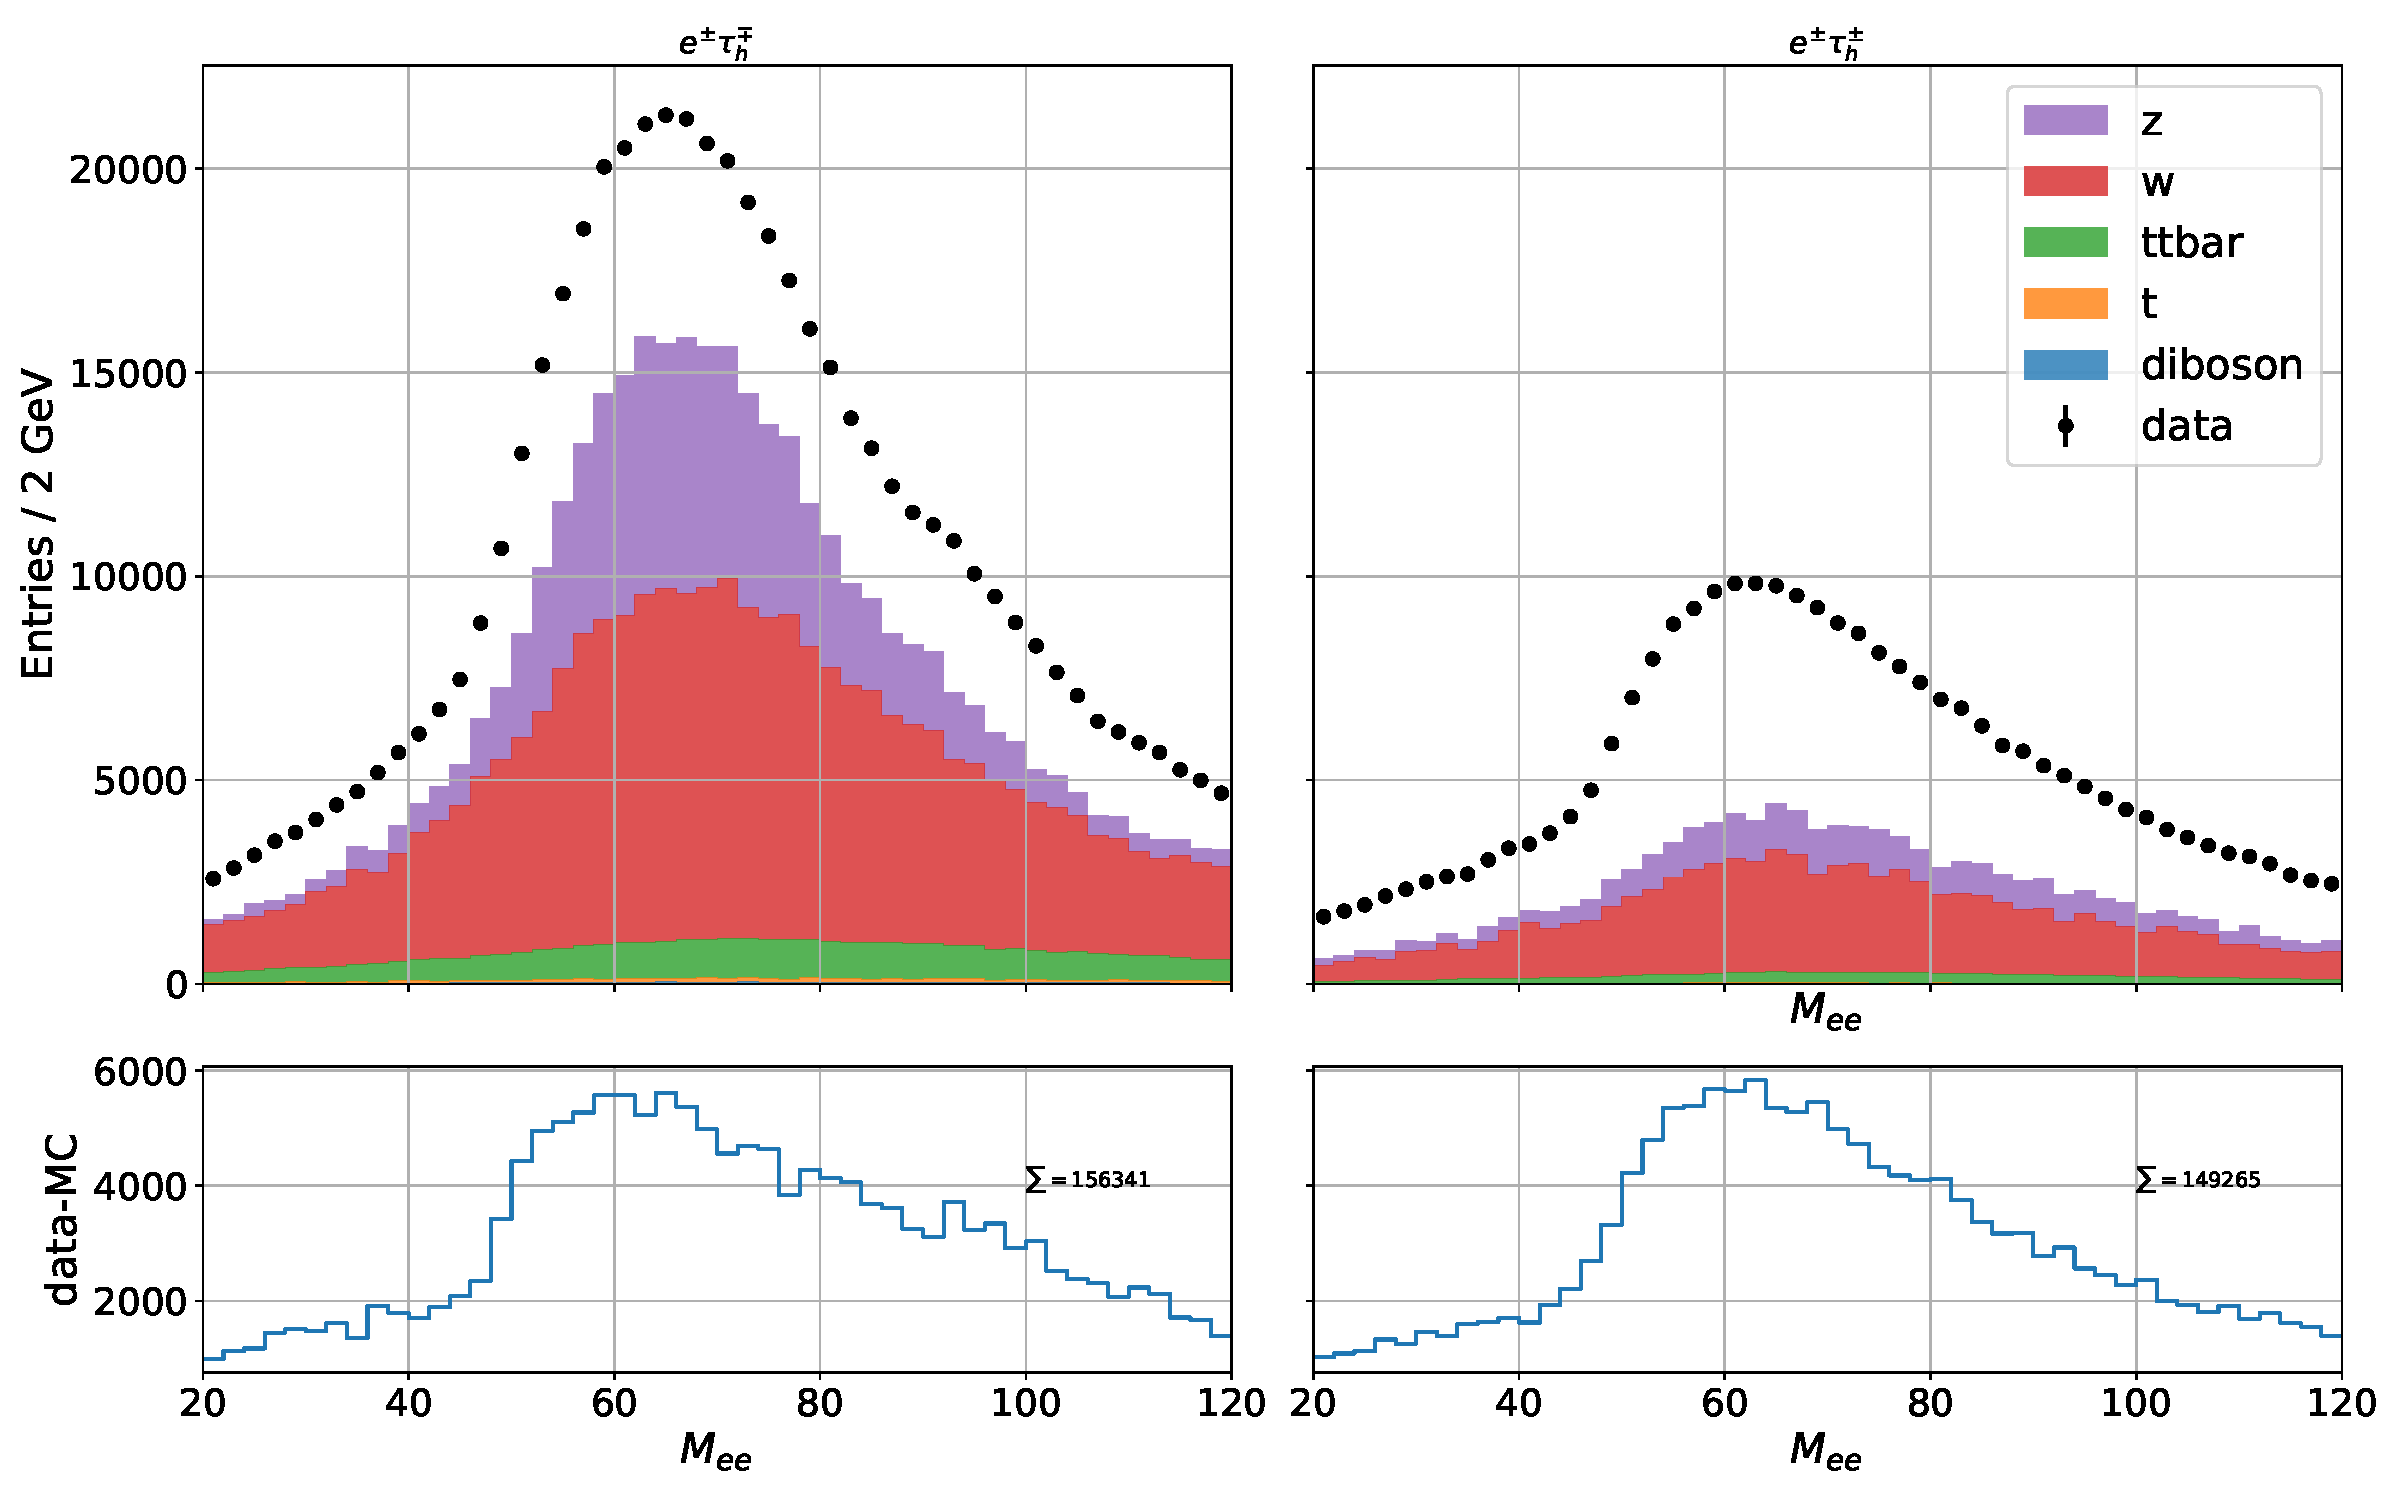
\includegraphics[width=0.7\textwidth]{chapters/Analysis/sectionBackground/figures/ltau_kinematics/etau_cr.pdf}
    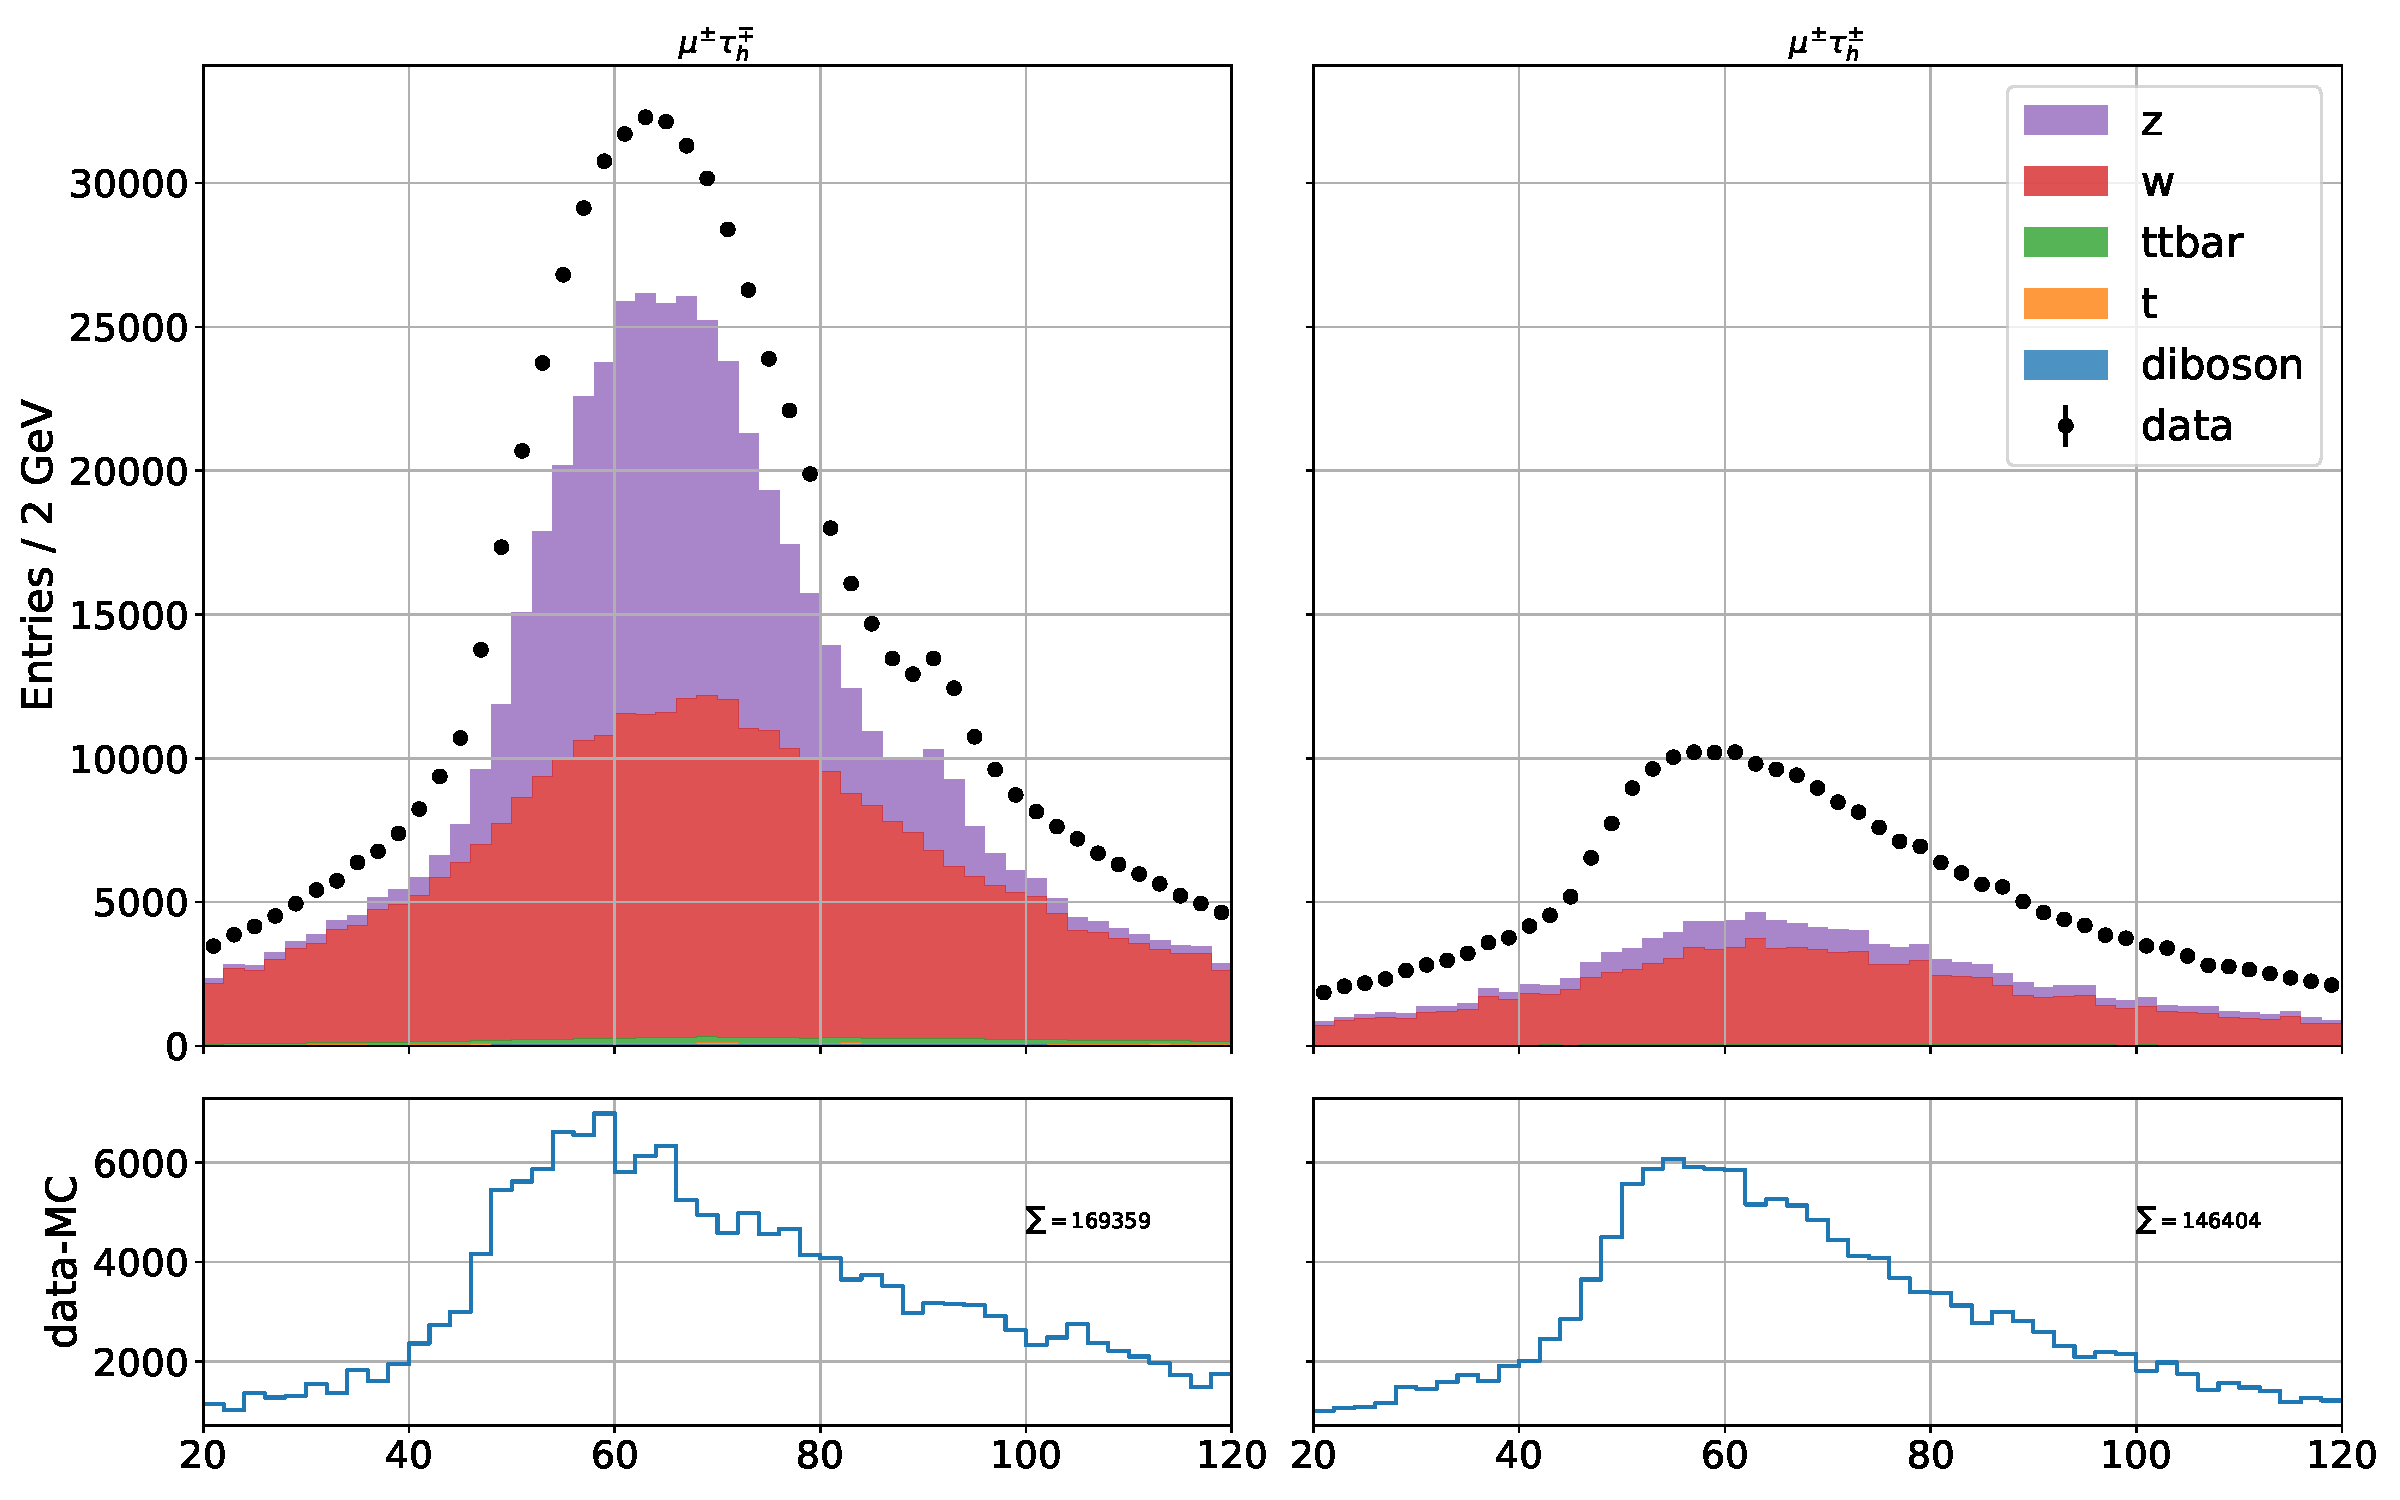
\includegraphics[width=0.7\textwidth]{chapters/Analysis/sectionBackground/figures/ltau_kinematics/mutau_cr.pdf}
    \caption{Opposite sign (left) and same sign (right) control regions for the \PZ enriched $e\tau$ (top) and $\mu\tau$ (bottom) selection.}
    \label{fig:ltau_fakes}
\end{figure}


In counting analysis, the QCD background in the $e\tau$ and $\mu\tau$ channel with $n_j\geq 2,n_b=1$ and
$n_j\geq 2,n_b\geq2$ is estimated with the QCD in the same-sign region scaled by a ss-to-os scale factor.
The scale factor can be defined as
\begin{equation}
    SF = \frac{N^{\rm{os}}_{\rm{data}} - \sum N^{\rm{os}}_{\rm{MC}} } {N^{\rm{ss}}_{\rm{data}} - \sum N^{\rm{ss}}_{\rm{MC}} }/
\end{equation}
\noindent The scale factor is derived from orthogonal $n_j,n_b$ regions.
Figure~\ref{fig:appendix:qcdsf:ltau, fig:appendix:qcdsf:ltau2} show the ss and os region of the $\mu\tau$ (left two columns) and 
$e\tau$ (right two columns) channel with different orthogonal $n_j,n_b$. Being the closest to the signal
$n_j,n_b$ category, the ss-to-os scale factor derived with $n_j\geq2,n_b=0$ is used to estimate the QCD 
background.


\begin{sidewaysfigure}[htb!]
    \centering
    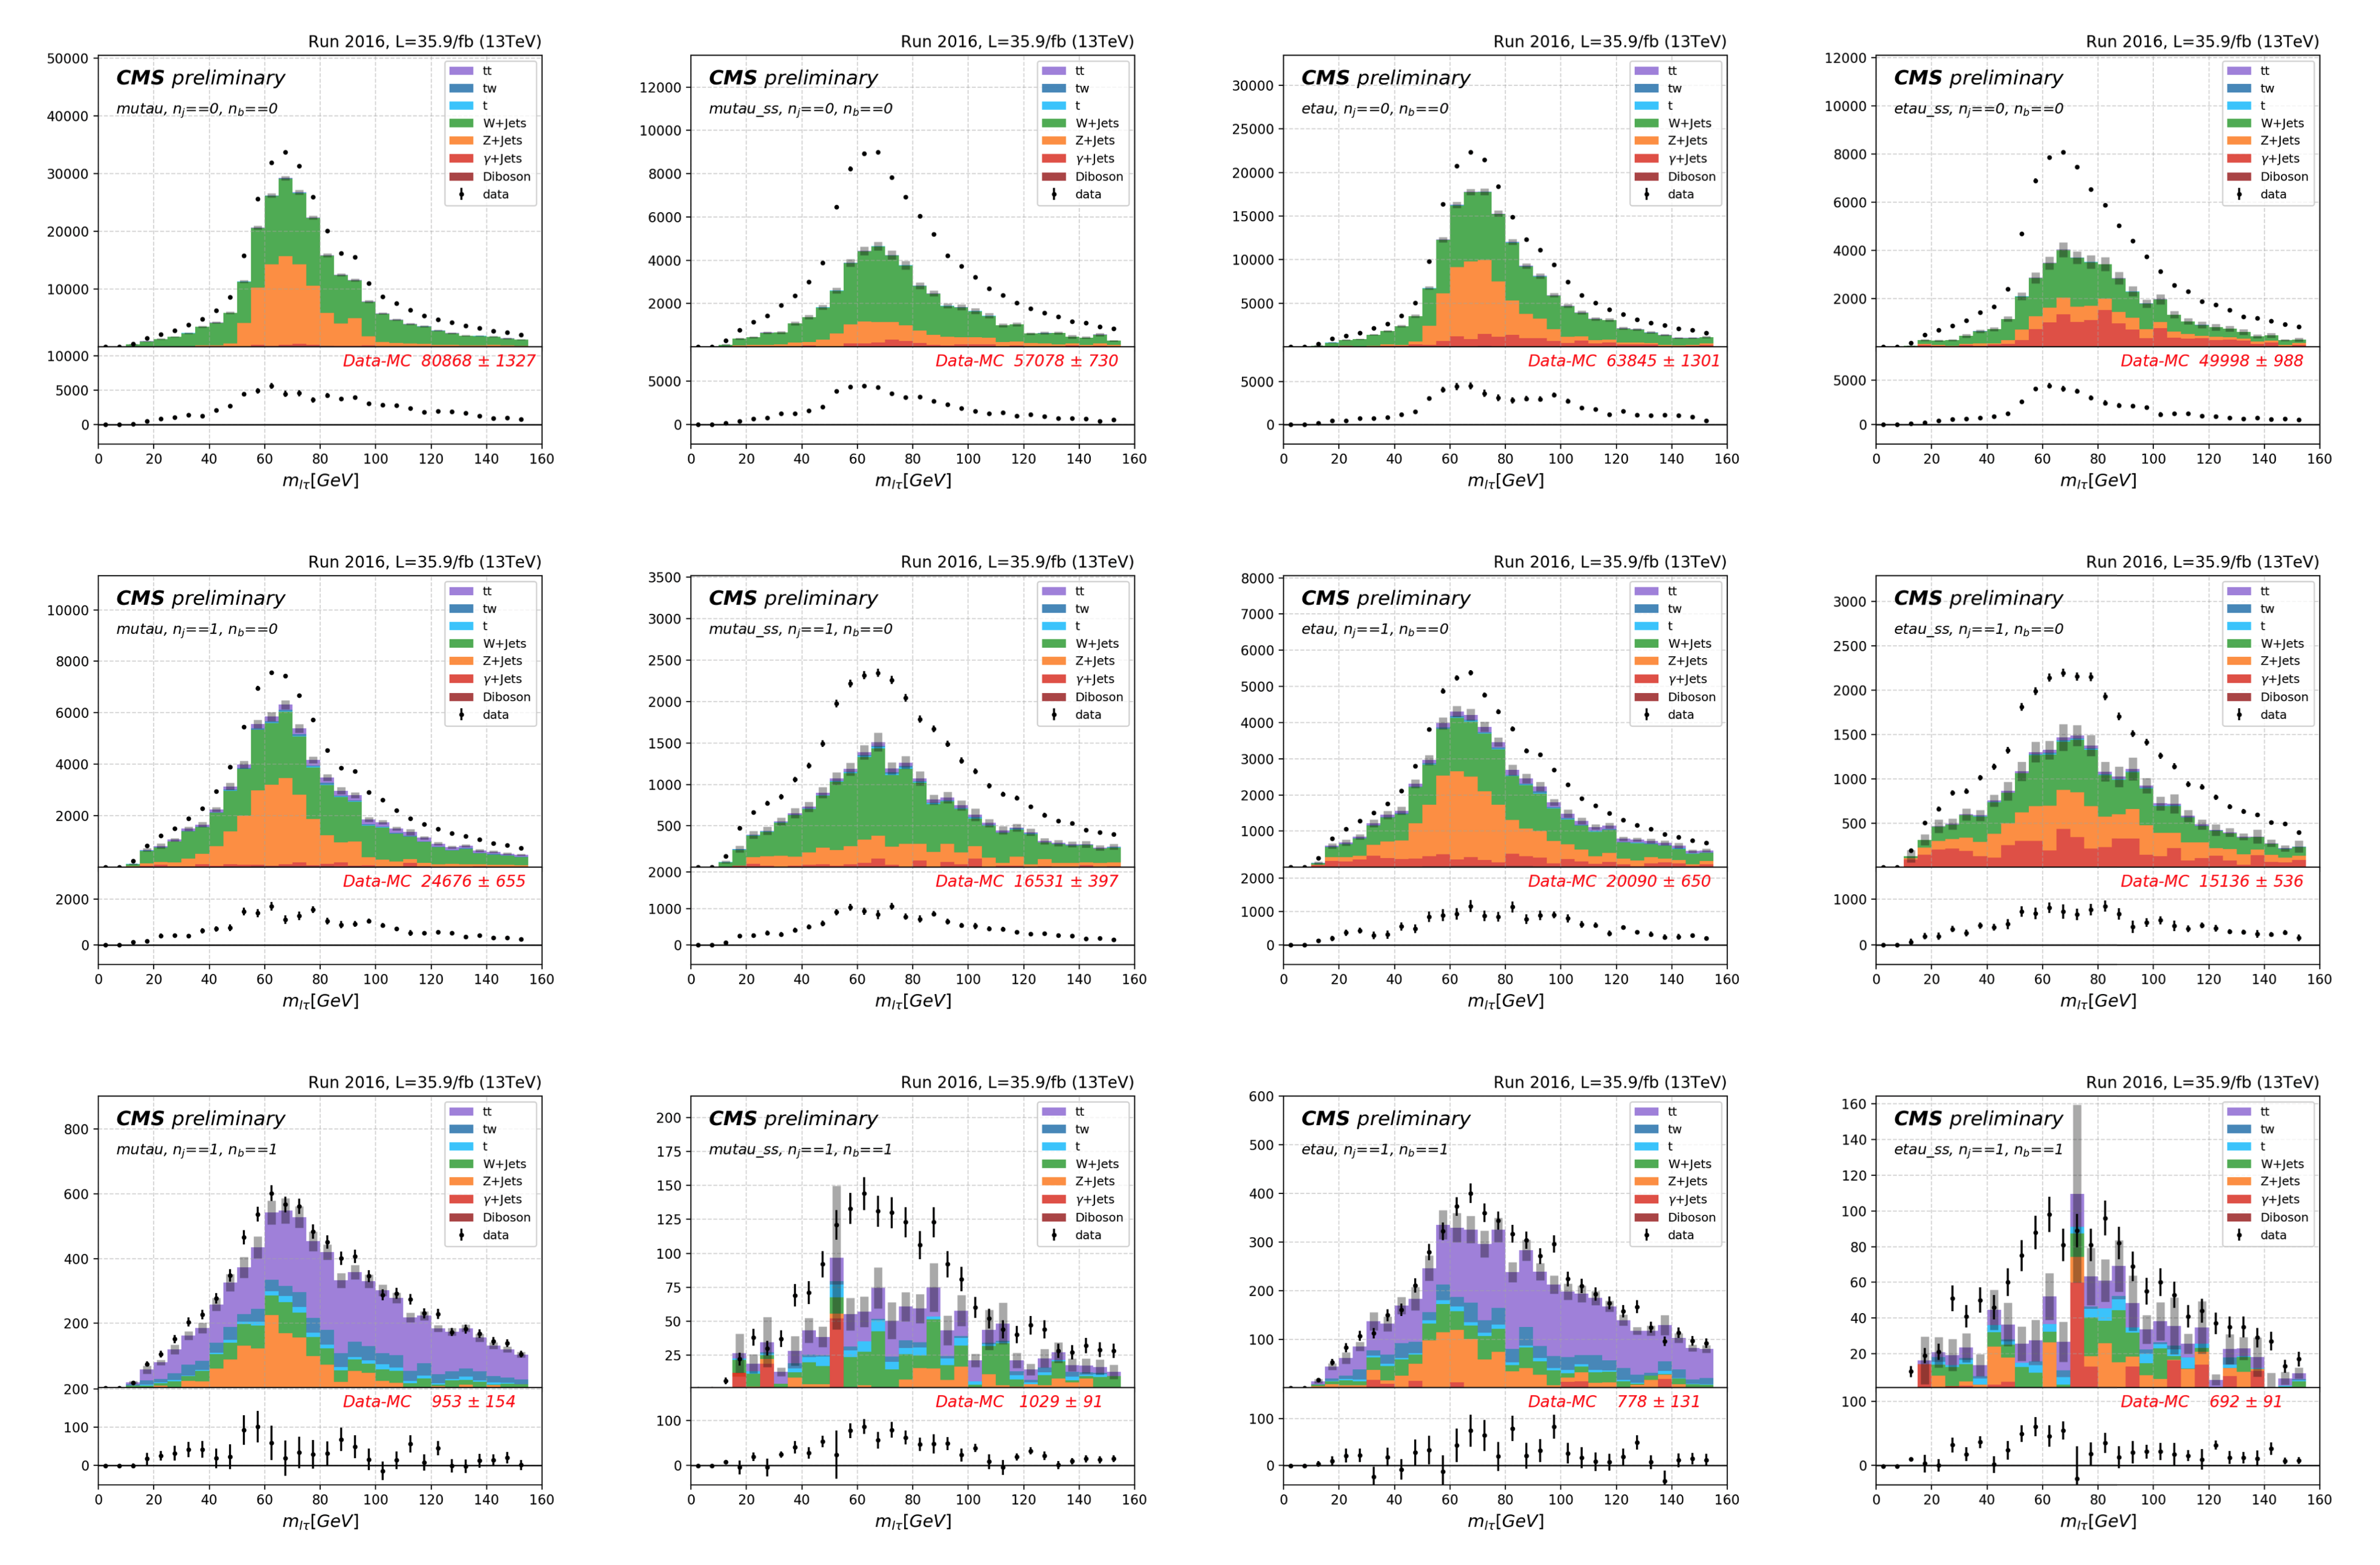
\includegraphics[width=0.9\textwidth]{chapters/Analysis/sectionBackground/figures/ltau_kinematics/ltau1.png}
    \caption{The $m_{l\tau}$ in the SS and OS region of $\mu\tau$ (left two columns) and $e\tau$ (right two columns) 
    channel. Different rows correspond to different $n_j,n_b$ configuration, which includes
    $n_j=0,n_b=0$, $n_j=1,n_b=0$, $n_j=1,n_b=1$. 
    }
    \label{fig:appendix:qcdsf:ltau}
\end{sidewaysfigure}



\begin{sidewaysfigure}[htb!]
    \centering
    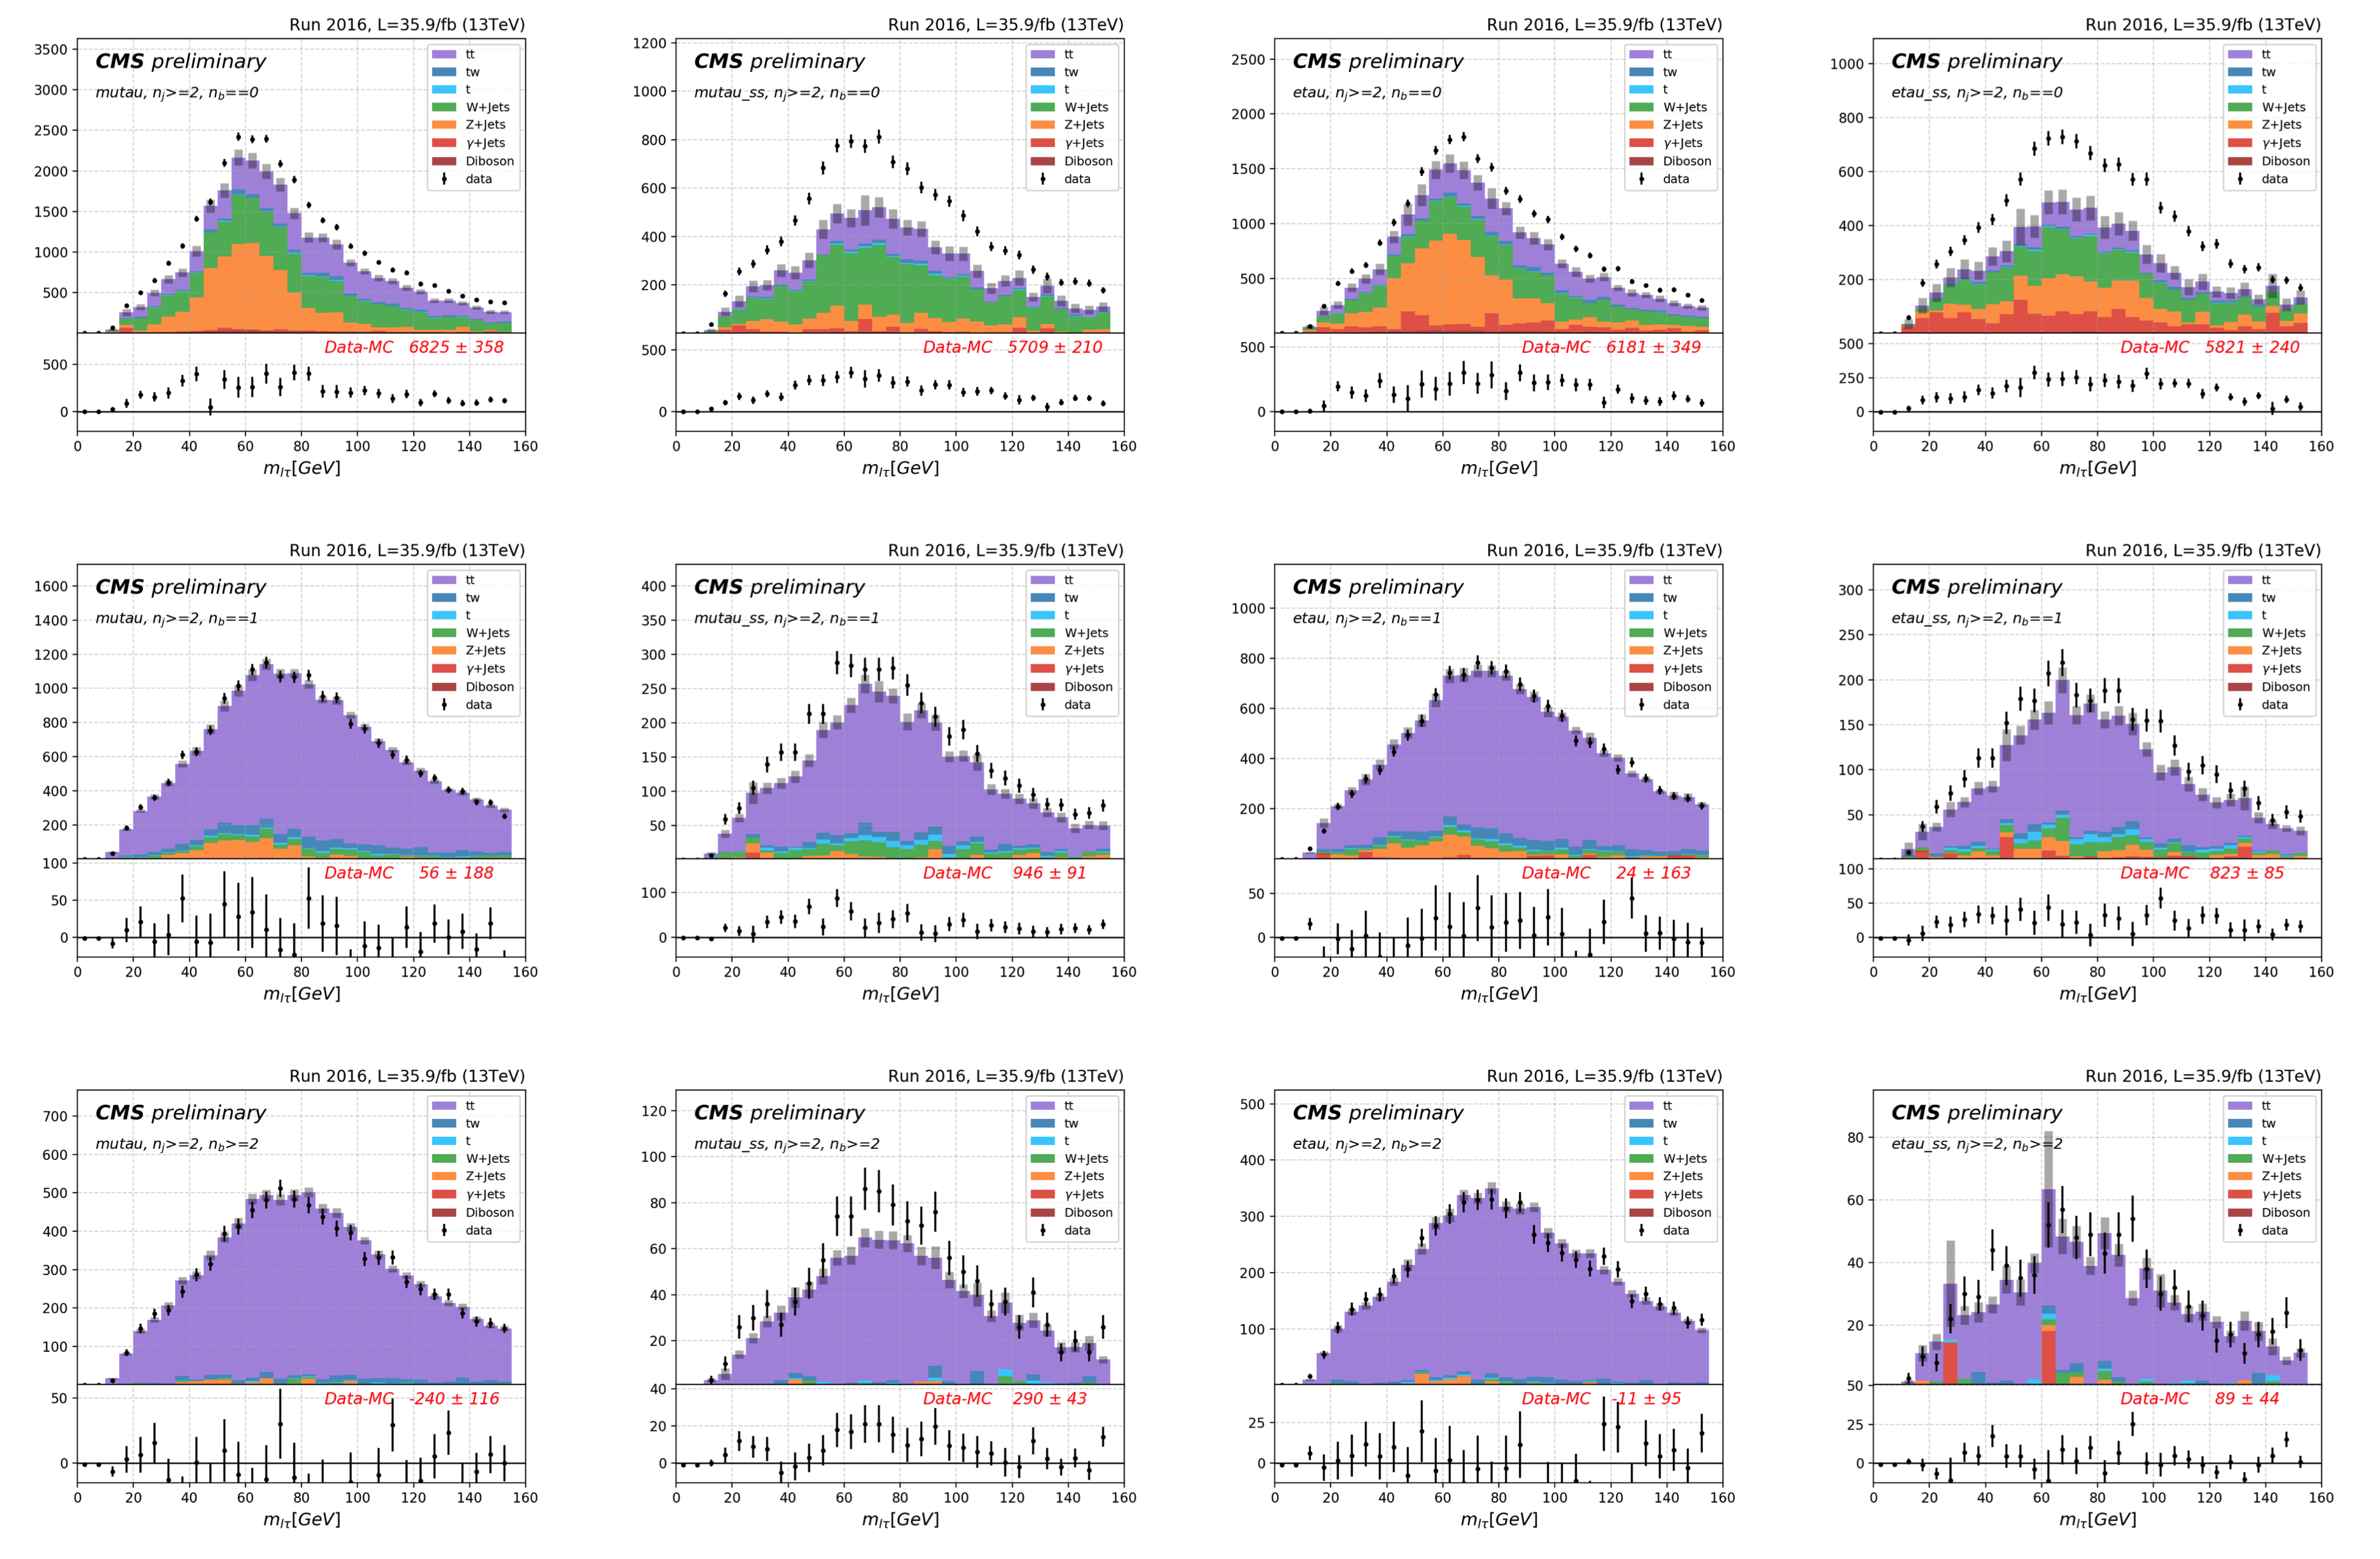
\includegraphics[width=0.9\textwidth]{chapters/Analysis/sectionBackground/figures/ltau_kinematics/ltau2.png}

    \caption{The $m_{l\tau}$ in the SS and OS region of $\mu\tau$ (left two columns) and $e\tau$ (right two columns) 
    channel. Different rows correspond to different $n_j,n_b$ configuration, which includes
    $n_j\geq 2,n_b=0$, $n_j\geq 2,n_b=1$, $n_j\geq 2,n_b\geq 2$. The last two rows dominated by \ttbar are the channels used by the counting analysis.
    }
    \label{fig:appendix:qcdsf:ltau2}
\end{sidewaysfigure}



\FloatBarrier


